\documentclass[11pt]{article}

% ---------- Codificación y tipografía ----------
\usepackage[utf8]{inputenc}
\usepackage[T1]{fontenc}
\usepackage{mathpazo}            % Palatino (texto + matemáticas)
\usepackage[protrusion=true,expansion=false]{microtype}

% ---------- Página ----------
\usepackage[a4paper,top=3cm,bottom=3cm,left=2.9cm,right=2.9cm]{geometry}
\usepackage{setspace}
\linespread{1.08}
\setlength{\emergencystretch}{3em}

% ---------- Matemáticas ----------
\usepackage{amsmath,amssymb,amsthm,mathtools}
\setlength{\jot}{7pt}
\allowdisplaybreaks
\renewcommand{\boxed}[1]{#1}     % sin recuadros alrededor de resultados

% ---------- Utilidades ----------
\usepackage{enumitem}
\setlist{itemsep=3pt,topsep=4pt,parsep=0pt}
\usepackage{booktabs}
\usepackage{needspace}
\usepackage{graphicx}
\usepackage{tikz}
\usetikzlibrary{arrows.meta,calc}
\usepackage{titlesec}
\usepackage{fancyhdr}
\usepackage[hidelinks]{hyperref}

% ---------- Párrafos ----------
\setlength{\parindent}{0pt}
\setlength{\parskip}{0.7em}

% ---------- Encabezados (estilo académico, monocromo) ----------
\renewcommand{\partname}{Parte}
\titleformat{\part}[display]
  {\normalfont\centering}
  {\large\scshape\partname~\thepart}
  {0.5em}
  {\huge\bfseries}
  [\vspace{2pt}{\titlerule[1pt]}]
\titlespacing*{\part}{0pt}{2.6ex plus 1ex}{2.4ex}

\titleformat{\section}[hang]
  {\normalfont\large\bfseries\scshape}{\thesection}{0.8em}{}
  [\vspace{2pt}{\titlerule[0.7pt]}]
\titlespacing*{\section}{0pt}{3.4ex plus 1ex minus .2ex}{2.0ex plus .2ex}

\titleformat{\subsection}[hang]
  {\normalfont\normalsize\bfseries}{\thesubsection}{0.7em}{}
\titlespacing*{\subsection}{0pt}{2.6ex plus 1ex}{1.1ex}

\titleformat{\subsubsection}[runin]
  {\normalfont\bfseries\itshape}{}{0pt}{}
\titlespacing*{\subsubsection}{0pt}{1.8ex plus 1ex}{0.8em}

% ---------- Encabezado de página ----------
\pagestyle{fancy}
\fancyhf{}
\renewcommand{\sectionmark}[1]{\markboth{\thesection.\ #1}{}}
\fancyhead[L]{\small\itshape\nouppercase{\leftmark}}
\fancyhead[R]{\small\thepage}
\renewcommand{\headrulewidth}{0.4pt}

% ---------- Bloques destacados (sin cajas, sólo entradilla en negrita) ----------
\newenvironment{clave}[1][Idea clave]%
  {\par\medskip\noindent\textbf{#1.}\enspace\ignorespaces}%
  {\par\medskip}
\newenvironment{notabox}[1][Nota]%
  {\par\medskip\noindent\textbf{#1.}\enspace\ignorespaces}%
  {\par\medskip}

% ---------- Teoremas ----------
\theoremstyle{definition}
\newtheorem{definicion}{Definición}[section]

% ---------- Comandos ----------
\newcommand{\E}{\mathbb{E}}
\newcommand{\dd}{\,\mathrm{d}}
\newcommand{\mc}{\mathrm{mc}}
\newcommand{\CP}{\mathrm{CP}}
\newcommand{\CM}{\mathrm{CM}}
\renewcommand{\contentsname}{Índice}

\hypersetup{pdftitle={Macroeconomía — Notas de clase}}

\begin{document}

\begin{titlepage}
\thispagestyle{empty}
\vspace*{3.5cm}
\begin{center}
\rule{\textwidth}{1pt}\\[1.1cm]
{\Huge\bfseries Macroeconomía}\\[0.6cm]
{\Large Notas de clase}\\[0.35cm]
{\large Josué David Fidel Cárdenas Barrantes}\\[1.0cm]
\rule{\textwidth}{1pt}
\end{center}
\vfill
\end{titlepage}

\newpage
\tableofcontents
\thispagestyle{empty}
\newpage
\setcounter{page}{1}

% ==========================================================
\part{Crecimiento}
% ==========================================================

\section{Crecimiento}

\subsection{Diagramas de fase: \emph{source}, \emph{sink} y \emph{saddle path}}

Para una dinámica escalar $\dot{x}=f(x)$: un \emph{source} es inestable (las flechas se alejan del
punto fijo) y un \emph{sink} es estable (convergen). Una variable de \textbf{estado} (p.\,ej.\ el
capital $k$) es predeterminada y hereda dinámica estable: $\dot{k}=f(k)$ converge a $k^{\ast}$ desde
cualquier $k_{0}$. Una variable de \textbf{control} (\emph{jump}, p.\,ej.\ el consumo) se elige cada
instante y requiere dinámica inestable para tener unicidad; si fuera estable habría multiplicidad de
equilibrios.

Para un sistema $(\dot{k},\dot{c})$ con \emph{loci} $\dot{k}=0$ y $\dot{c}=0$:
\begin{itemize}[leftmargin=1.4em]
\item \textbf{Source} (ambos divergen): cualquier punto expulsa del equilibrio.
\item \textbf{Sink} (ambos convergen): cualquier $c$ lleva al equilibrio $\Rightarrow$ indeterminación.
\item \textbf{Saddle path}: una dirección estable (variable de estado $k$) y una inestable (control $c$).
Sólo una trayectoria lleva al equilibrio; hay un único $c_{0}$ compatible. Congruencia: variables de
estado $\leftrightarrow$ dinámica estable; variables de control $\leftrightarrow$ dinámica inestable.

\begin{figure}[h]
\centering
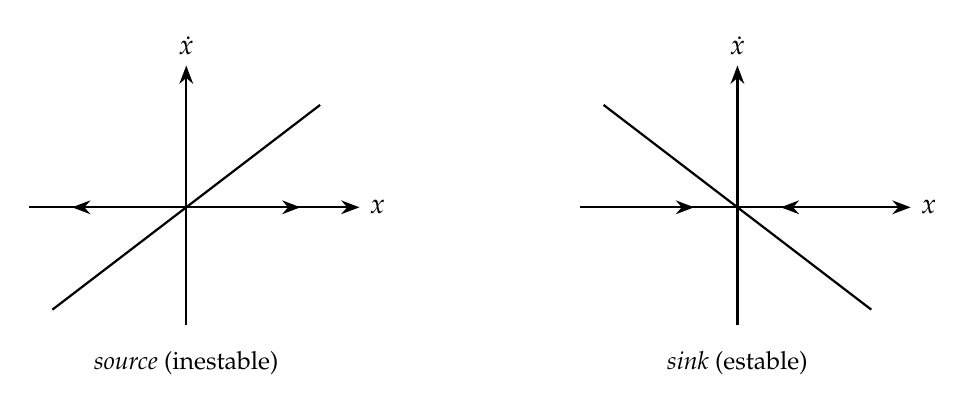
\begin{tikzpicture}[>=Stealth,line width=0.8pt]
  \begin{scope}
    \draw[->] (-2,0)--(2.2,0) node[right]{$x$};
    \draw[->] (0,-1.5)--(0,1.8) node[above]{$\dot{x}$};
    \draw (-1.7,-1.3)--(1.7,1.3);
    \draw[->] (0.5,0)--(1.45,0);
    \draw[->] (-0.5,0)--(-1.45,0);
    \node[below] at (0,-1.7){\small\emph{source} (inestable)};
  \end{scope}
  \begin{scope}[xshift=7cm]
    \draw[->] (-2,0)--(2.2,0) node[right]{$x$};
    \draw[->] (0,-1.5)--(0,1.8) node[above]{$\dot{x}$};
    \draw (-1.7,1.3)--(1.7,-1.3);
    \draw[->] (1.45,0)--(0.55,0);
    \draw[->] (-1.45,0)--(-0.55,0);
    \node[below] at (0,-1.7){\small\emph{sink} (estable)};
  \end{scope}
\end{tikzpicture}
\caption{Dinámica escalar $\dot{x}=f(x)$: un \emph{source} repele (las flechas se alejan del punto
fijo) y un \emph{sink} atrae (convergen).}
\end{figure}

\begin{figure}[h]
\centering
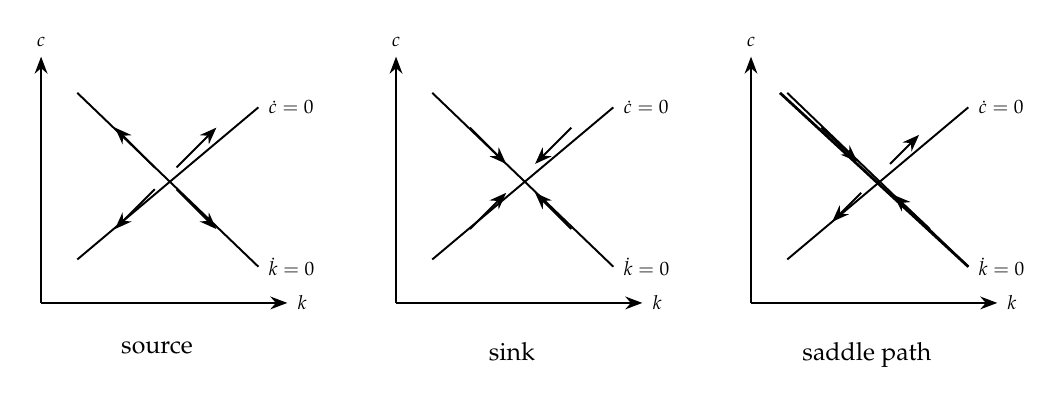
\begin{tikzpicture}[>=Stealth,line width=0.7pt,scale=0.92]
  % --- source ---
  \begin{scope}
    \draw[->](0,0)--(3.4,0) node[right]{\scriptsize $k$};
    \draw[->](0,0)--(0,3.4) node[above]{\scriptsize $c$};
    \draw (0.5,0.6)--(3.0,2.7); \node[right] at (3.0,2.7){\scriptsize $\dot{c}=0$};
    \draw (0.5,2.9)--(3.0,0.5); \node[right] at (3.0,0.5){\scriptsize $\dot{k}=0$};
    \coordinate (S) at (1.72,1.72);
    \draw[->](S)++(0.15,0.15)--++(0.55,0.55);
    \draw[->](S)++(-0.15,0.15)--++(-0.55,0.55);
    \draw[->](S)++(0.15,-0.15)--++(0.55,-0.55);
    \draw[->](S)++(-0.15,-0.15)--++(-0.55,-0.55);
    \node[below] at (1.6,-0.4){\small source};
  \end{scope}
  % --- sink ---
  \begin{scope}[xshift=4.9cm]
    \draw[->](0,0)--(3.4,0) node[right]{\scriptsize $k$};
    \draw[->](0,0)--(0,3.4) node[above]{\scriptsize $c$};
    \draw (0.5,0.6)--(3.0,2.7); \node[right] at (3.0,2.7){\scriptsize $\dot{c}=0$};
    \draw (0.5,2.9)--(3.0,0.5); \node[right] at (3.0,0.5){\scriptsize $\dot{k}=0$};
    \coordinate (S) at (1.72,1.72);
    \draw[->]($(S)+(0.7,0.7)$)--($(S)+(0.2,0.2)$);
    \draw[->]($(S)+(-0.7,0.7)$)--($(S)+(-0.2,0.2)$);
    \draw[->]($(S)+(0.7,-0.7)$)--($(S)+(0.2,-0.2)$);
    \draw[->]($(S)+(-0.7,-0.7)$)--($(S)+(-0.2,-0.2)$);
    \node[below] at (1.6,-0.4){\small sink};
  \end{scope}
  % --- saddle ---
  \begin{scope}[xshift=9.8cm]
    \draw[->](0,0)--(3.4,0) node[right]{\scriptsize $k$};
    \draw[->](0,0)--(0,3.4) node[above]{\scriptsize $c$};
    \draw (0.5,0.6)--(3.0,2.7); \node[right] at (3.0,2.7){\scriptsize $\dot{c}=0$};
    \draw (0.5,2.9)--(3.0,0.5); \node[right] at (3.0,0.5){\scriptsize $\dot{k}=0$};
    \coordinate (S) at (1.72,1.72);
    \draw[line width=1pt] (0.4,2.9)--(3.0,0.5);
    \draw[->]($(S)+(-0.75,0.7)$)--($(S)+(-0.25,0.23)$);
    \draw[->]($(S)+(0.75,-0.7)$)--($(S)+(0.25,-0.23)$);
    \draw[->]($(S)+(0.2,0.2)$)--($(S)+(0.6,0.6)$);
    \draw[->]($(S)+(-0.2,-0.2)$)--($(S)+(-0.6,-0.6)$);
    \node[below] at (1.6,-0.4){\small saddle path};
  \end{scope}
\end{tikzpicture}
\caption{Retratos de fase del sistema $(\dot{k},\dot{c})$. \emph{Source}: ambas dinámicas divergen.
\emph{Sink}: ambas convergen (indeterminación). \emph{Saddle path}: una dirección estable y una
inestable; sólo la trayectoria estable (línea gruesa) lleva al estado estacionario, y hay un único
$c_{0}$ compatible.}
\end{figure}

\end{itemize}

\subsection{Modelo de Solow}

En términos per cápita ($n$ = crecimiento poblacional, $\delta$ = depreciación),
\begin{equation}
\dot{k}=\frac{\mathrm{d}(K/L)}{\mathrm{d}t}=\frac{\dot{K}}{L}-nk,
\qquad\qquad
\dot{k}=s\,f(k)-(n+\delta)k .
\end{equation}
$k$ es variable de estado ($k_{0}$ dado). El modelo \emph{no} genera crecimiento; sólo muestra cómo
se converge al equilibrio
\begin{equation}
s\,f(k^{\ast})=(n+\delta)k^{\ast}\qquad\text{(condición de equilibrio).}
\end{equation}

\begin{figure}[h]
\centering
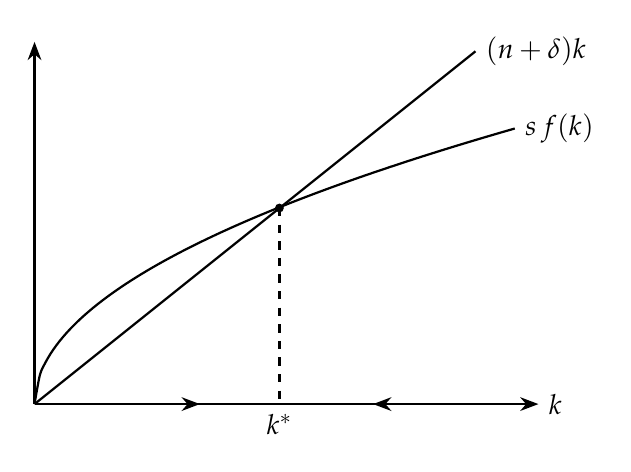
\begin{tikzpicture}[>=Stealth,line width=0.8pt]
  \draw[->](0,0)--(6.4,0) node[right]{$k$};
  \draw[->](0,0)--(0,4.6);
  % (n+delta)k
  \draw (0,0)--(5.6,4.48); \node[right] at (5.6,4.48){$(n+\delta)k$};
  % s f(k)
  \draw[domain=0:6.1,samples=90,smooth] plot(\x,{3.5*sqrt(\x)/sqrt(6.1)});
  \node[right] at (6.1,{3.5*sqrt(6.1)/sqrt(6.1)}){$s\,f(k)$};
  % k*
  \coordinate (K) at (3.11,2.49);
  \draw[dashed] (3.11,2.49)--(3.11,0) node[below]{$k^{\ast}$};
  \fill (3.11,2.49) circle (1.6pt);
  % convergence arrows
  \draw[->](1.2,0)--(2.1,0);
  \draw[->](5.2,0)--(4.3,0);
\end{tikzpicture}
\caption{Modelo de Solow. El capital converge a $k^{\ast}$, donde $s\,f(k^{\ast})=(n+\delta)k^{\ast}$;
el modelo no genera crecimiento de largo plazo, sólo dinámica de transición.}
\end{figure}

Con $y=Ak^{\alpha}$, resolviendo $sAk^{\ast\alpha}=(n+\delta)k^{\ast}$,
\begin{equation}
k^{\ast}=\Big(\frac{sA}{n+\delta}\Big)^{\frac{1}{1-\alpha}},
\qquad
y^{\ast}=A^{\frac{1}{1-\alpha}}\Big(\frac{s}{n+\delta}\Big)^{\frac{\alpha}{1-\alpha}} .
\end{equation}
Comparando países,
\begin{equation}
\frac{y_{1}}{y_{2}}=\Big(\frac{A_{1}}{A_{2}}\Big)^{\frac{1}{1-\alpha}}\Big(\frac{s_{1}}{s_{2}}\Big)^{\frac{\alpha}{1-\alpha}} :
\end{equation}
En este sentido, la tecnología es muy importante para comprender las diferencias de ingreso.

\subsection{Problema de Ramsey}

\begin{equation}
\max\ \int_{0}^{\infty}U(C_{t})\,e^{-\rho t}\dd t,\qquad \rho=\text{impaciencia},
\qquad\qquad
\dot{k}=f(k)-nk-c .
\end{equation}
Con el hamiltoniano $H=U(C_{t})e^{-\rho t}+\mu_{t}[f(k)-nk-c_{t}]$, las CPO son
\begin{align}
&U'(C_{t})e^{-\rho t}-\mu_{t}=0, \\
&\dot{\mu}_{t}=-\mu_{t}\big[f'(k_{t})-n\big], \\
&\lim_{t\to\infty}k_{t}\mu_{t}e^{-\rho t}=0\quad\text{(TVC).}
\end{align}
Definiendo el valor corriente $\lambda_{t}=\mu_{t}e^{\rho t}$ (con
$\dot{\lambda}_{t}/\lambda_{t}=\dot{\mu}_{t}/\mu_{t}+\rho$),
\begin{equation}
U'(C_{t})=\lambda_{t},
\qquad
\frac{\dot{\lambda}_{t}}{\lambda_{t}}=\rho+n-f'(k_{t}),
\qquad
\lim_{t\to\infty}k_{t}\lambda_{t}e^{-\rho t}=0 .
\end{equation}
Diferenciando $U'(C_{t})=\lambda_{t}$ y definiendo la elasticidad de sustitución intertemporal
$\sigma=-\dfrac{U'(C_{t})}{U''(C_{t})C_{t}}>0$, se obtiene la \textbf{Euler en tiempo continuo}:
\begin{equation}
\boxed{\ \frac{\dot{C}_{t}}{C_{t}}=\sigma\big(f'(k_{t})-\rho-n\big)\ }.
\end{equation}
La pendiente del consumo depende de la diferencia entre $f'(k)$ (tasa de interés) y $\rho$
(descuento): si es positiva, se ahorra más, baja el consumo hoy, se acumula capital y el consumo
crece en el tiempo. Es una ecuación de arbitraje, con $\lambda$ el costo de oportunidad del capital.

\subsubsection{Diagrama de fase de Ramsey}
\begin{equation}
\dot{k}=0:\quad C^{\ast}=f(k^{\ast})-nk^{\ast}\ \ \text{(factibilidad)};
\qquad\qquad
\dot{C}=0:\quad f'(k^{\ast})=\rho+n\ \ \text{(Euler).}
\end{equation}

\begin{figure}[h]
\centering
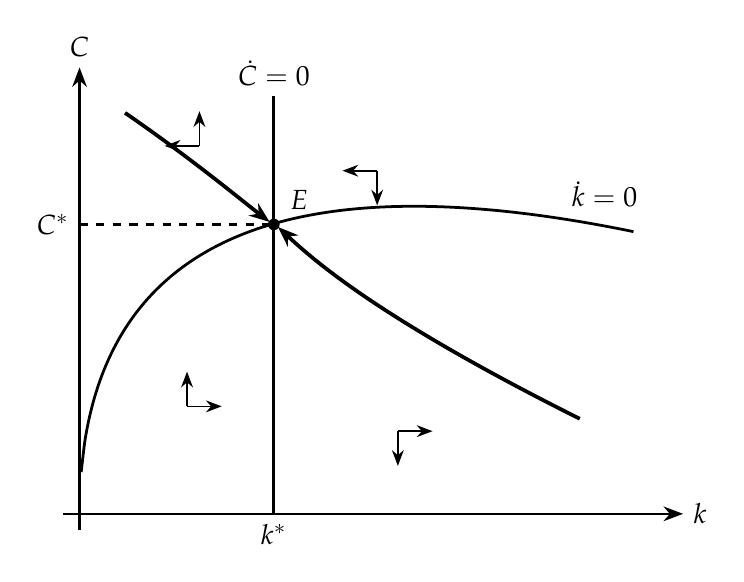
\begin{tikzpicture}[>=Stealth,line width=0.9pt,scale=1.05]
  % ejes
  \draw[->](-0.2,0)--(7.3,0) node[right]{$k$};
  \draw[->](0,-0.2)--(0,5.4) node[above]{$C$};
  % locus kdot=0 (joroba)
  \draw[line width=1pt,domain=0.02:6.7,samples=160,smooth] plot(\x,{3.7*sqrt(\x)-0.92*\x});
  \node[above] at (6.35,{3.7*sqrt(6.35)-0.92*6.35+0.1}){$\dot{k}=0$};
  % locus Cdot=0 (vertical)
  \draw[line width=1pt](2.35,0)--(2.35,5.05); \node[above] at (2.35,5.05){$\dot{C}=0$};
  \draw[dashed](2.35,0)node[below]{$k^{\ast}$}--(2.35,3.50);
  \draw[dashed](0,3.50)node[left]{$C^{\ast}$}--(2.35,3.50);
  % estado estacionario
  \fill (2.35,3.50) circle (2pt); \node[above right] at (2.42,3.55){$E$};
  % rama estable (saddle path) con flechas hacia E
  \draw[line width=1.35pt,-{Stealth[length=2.6mm]}] (0.55,4.85) .. controls (1.35,4.30) and (1.95,3.80) .. (2.30,3.53);
  \draw[line width=1.35pt,-{Stealth[length=2.6mm]}] (6.05,1.15) .. controls (3.65,2.35) and (2.85,3.05) .. (2.40,3.47);
  % campo de direcciones en las 4 regiones (flechas finas)
  \begin{scope}[line width=0.6pt]
    \draw[->](1.30,1.30)--(1.72,1.30); \draw[->](1.30,1.30)--(1.30,1.72); % SO: k+, C+
    \draw[->](1.45,4.45)--(1.03,4.45); \draw[->](1.45,4.45)--(1.45,4.87); % NO: k-, C+
    \draw[->](3.85,1.00)--(4.27,1.00); \draw[->](3.85,1.00)--(3.85,0.58); % SE: k+, C-
    \draw[->](3.60,4.15)--(3.18,4.15); \draw[->](3.60,4.15)--(3.60,3.73); % NE: k-, C-
  \end{scope}
\end{tikzpicture}
\caption{Diagrama de fase de Ramsey--Cass--Koopmans. La curva $\dot{k}=0$ es $C=f(k)-nk$
(factibilidad) y la vertical $\dot{C}=0$ está en $f'(k^{\ast})=\rho+n$ (Euler). Las flechas finas
muestran el campo de direcciones en cada región; el estado estacionario $E$ es un punto de silla y sólo
la rama estable (línea gruesa, con flechas hacia $E$) lo alcanza. Las demás trayectorias violan la
condición de transversalidad.}
\end{figure}

El sistema es un \textbf{saddle path}: sólo un $C_{0}$ converge; las demás trayectorias violan la
TVC. Al linealizar alrededor del \emph{steady state},
$[\dot{k}_{t},\dot{C}_{t}]'=\Omega\,[k_{t}-k^{\ast},\,C_{t}-C^{\ast}]'$, la solución se comporta como
$A e^{\lambda_{1}t}+B e^{\lambda_{2}t}$; se impone $B=0$ (vía la variable de control) para satisfacer
la TVC. Como $\det(\Omega)=\sigma C^{\ast}f''(k^{\ast})<0$, hay un autovalor positivo y uno negativo:
\emph{saddle path}, con unicidad (una variable \emph{jump} requiere un autovalor inestable, à la
Blanchard--Kahn). No puede ser un \emph{sink} (daría indeterminación). El consumo es \emph{jump
variable}: no está determinado por una ecuación de acumulación, se elige cada instante resolviendo un
problema intertemporal y es \emph{forward looking}. La regla dorada de este modelo es menor que en
Solow ($\rho>n$): al descontar el futuro, es óptimo consumir más en la transición al BGP y desaparece
la posibilidad de sobre-ahorro. A continuación se construye el diagrama panel por panel y se formaliza la estabilidad.

\paragraph{Construcción del diagrama de fase.} El \emph{locus} $\dot{k}=0$ da la condición de
factibilidad $C^{\ast}=f(k^{\ast})-nk^{\ast}$ (si $k\uparrow$ entonces $C^{\ast}\downarrow$ a la
derecha del máximo), con $\dot{k}>0$ por debajo de la joroba y $\dot{k}<0$ por encima. El \emph{locus}
$\dot{C}=0$ es la vertical $f'(k^{\ast})=\rho+n$ (Euler): cuando $k<k^{\ast}$ la productividad marginal
es alta ($f'(k)>\rho+n$) y el consumo crece ($\dot{C}>0$), y viceversa.

\begin{figure}[h]
\centering
\begin{tikzpicture}[>=Stealth,line width=0.85pt]
  % panel 1: kdot=0
  \begin{scope}
    \draw[->](0,0)--(5.4,0) node[right]{$k$};
    \draw[->](0,0)--(0,3.6) node[above]{$C$};
    \draw[domain=0.05:5.0,samples=100,smooth] plot(\x,{2.9*sqrt(\x)-0.72*\x});
    \node[right] at (4.4,{2.9*sqrt(4.4)-0.72*4.4}){$\dot{k}=0$};
    \draw[->](1.0,2.55)--(0.55,2.55); \node[above] at (0.95,2.6){\scriptsize $\dot{k}<0$};
    \draw[->](2.2,1.05)--(2.65,1.05); \node[below] at (2.2,1.0){\scriptsize $\dot{k}>0$};
  \end{scope}
  % panel 2: Cdot=0
  \begin{scope}[xshift=7.2cm]
    \draw[->](0,0)--(5.4,0) node[right]{$k$};
    \draw[->](0,0)--(0,3.6) node[above]{$C$};
    \draw (2.2,0)node[below]{$k^{\ast}$}--(2.2,3.4); \node[above] at (2.2,3.4){$\dot{C}=0$};
    \draw[->](1.3,1.7)--(1.3,2.15); \node[left] at (1.25,1.9){\scriptsize $\dot{C}>0$};
    \draw[->](3.1,1.7)--(3.1,1.25); \node[right] at (3.15,1.9){\scriptsize $\dot{C}<0$};
  \end{scope}
\end{tikzpicture}
\caption{Construcción del diagrama de Ramsey. Izquierda: \emph{locus} $\dot{k}=0$ (factibilidad).
Derecha: \emph{locus} $\dot{C}=0$ (Euler). Su superposición produce el punto de silla de la Figura
anterior.}
\end{figure}

\paragraph{Linealización y condiciones de Blanchard--Kahn.} Hay variables de estado (predeterminadas,
$k$) y de control (\emph{jump}, $C$). Linealizando alrededor del \emph{steady state},
\begin{equation}
\begin{bmatrix}\dot{k}_{t}\\ \dot{C}_{t}\end{bmatrix}
=\Omega\begin{bmatrix}k_{t}-k^{\ast}\\ C_{t}-C^{\ast}\end{bmatrix},
\qquad
\Omega=\begin{bmatrix}\rho-n & -1\\[2pt] \sigma C^{\ast}f''(k^{\ast}) & 0\end{bmatrix}.
\end{equation}
El sistema se comporta como $A e^{\lambda_{1}t}+B e^{\lambda_{2}t}$: si $\lambda<0$ converge, si
$\lambda>0$ explota, y si $\lambda_{1}>0$ y $\lambda_{2}<0$ existe un \emph{saddle path}. Como
$\det(\Omega)=\sigma C^{\ast}f''(k^{\ast})<0$, hay un autovalor positivo y uno negativo: es un punto de
silla. No puede ser un \emph{sink}, pues tendríamos $\lambda_{1},\lambda_{2}<0$ e infinitos equilibrios
(no unicidad). Se impone $B=0$ (usando la variable de control) para satisfacer la TVC.
\begin{itemize}[leftmargin=1.4em]
\item Con \textbf{1 variable \emph{forward looking}} se necesita \textbf{1 autovalor positivo} para
unicidad (número de \emph{jumps} $=$ número de autovalores inestables).
\item En general debe haber una dirección estable ($\lambda<0$) y una explosiva ($\lambda>0$); el
coeficiente del término explosivo debe ser $0$ para no explotar. Las variables \emph{jump} existen
justamente para cancelar las fuerzas explosivas.
\item \textbf{Indeterminación} $\to$ infinitas trayectorias (ambos \emph{sink});
\textbf{inestabilidad} $\to$ sistema explosivo (ambos \emph{source}).
\end{itemize}
Notas del modelo: dentro de Ramsey \emph{no} hay ineficiencia dinámica como en Solow; la regla dorada
es menor que en Solow ($\rho>n$); la posibilidad de sobre-ahorro desaparece cuando los agentes son
optimizadores, porque el futuro está descontado y es óptimo consumir más en la transición al BGP. En
este modelo sólo se observa la dinámica transicional: en el BGP no hay crecimiento.

En tiempo discreto, con $A_{t+1}=R_{t}A_{t}+y_{t}-C_{t}$, la Euler es
$\beta\,\E_{t}[R_{t+1}U'(C_{t+1})]=U'(C_{t})$, isomorfa a la valuación
$P_{t}(1+r_{t})=P_{t+1}+d_{t}\Rightarrow P_{t}=\sum_{i\ge0}\dfrac{d_{t+i}}{(1+r)^{i+1}}$.

\subsection{Modelo AK (crecimiento endógeno)}

Se cambia la función de producción a $Y_{t}=AK_{t}$ (con $A>0$), $\dot{K}_{t}=AK_{t}-C_{t}$. Con
$H=\dfrac{\sigma}{\sigma-1}C_{t}^{\frac{\sigma-1}{\sigma}}+\lambda_{t}(AK_{t}-C_{t})$, las CPO son
$C_{t}^{-1/\sigma}=\lambda_{t}$ y $\dot{\lambda}_{t}=(\rho-A)\lambda_{t}$. Tomando derivadas respecto
al tiempo,
\begin{equation}
-\frac{1}{\sigma}\frac{\dot{C}_{t}}{C_{t}}=\frac{\dot{\lambda}_{t}}{\lambda_{t}}=\rho-A
\qquad\Longrightarrow\qquad
\boxed{\ \frac{\dot{C}_{t}}{C_{t}}=\sigma(A-\rho)\ }
\end{equation}
(la productividad marginal $f'(k)=A$ es ahora constante). Ésta es la tasa de crecimiento de la
economía: el consumo crece siempre. En el BGP,
\begin{equation}
\frac{\dot{C}_{t}}{C_{t}}=\frac{\dot{K}_{t}}{K_{t}}=\frac{\dot{y}_{t}}{y_{t}}=\sigma(A-\rho),
\qquad
C_{t}=\big[(1-\sigma)A+\sigma\rho\big]K_{t}=\frac{(1-\sigma)A+\sigma\rho}{A}\,y_{t}:
\end{equation}
el consumo es una proporción del ingreso. La economía crece de manera permanente y \textbf{los choques
temporales tienen efectos permanentes} (no hay dinámica transicional). Resolviendo la ecuación
diferencial, $C_{t}=C_{0}e^{\sigma(A-\rho)t}$ y $K_{t}=K_{0}e^{\sigma(A-\rho)t}$; la TVC
$\lim_{t\to\infty}K_{t}C_{t}^{-1/\sigma}e^{-\rho t}=0$ se reduce a
$\lim_{t\to\infty}K_{0}C_{0}^{-1/\sigma}e^{-\theta t}=0$, que exige $\theta>0$ con
\begin{equation}
\theta=(1-\sigma)A+\sigma\rho\qquad(\text{si }\sigma=1,\ \theta=\rho:\text{ caso logarítmico}).
\end{equation}

\begin{figure}[h]
\centering
\begin{tikzpicture}[>=Stealth,line width=0.85pt]
  \draw[->](0,0)--(8.4,0) node[right]{$t$};
  \draw[->](0,0)--(0,4.6) node[above]{$\ln C$};
  % sendero base (BGP) punteado
  \draw[dashed] (0,0.7)--(8,4.3);
  % sendero con choque temporal -> efecto permanente (nivel desplazado)
  \draw (0,0.7)--(2.6,1.87)                              % coincide con base hasta t1
        (2.6,1.87)--(3.1,2.55)                           % salto durante choque
        (3.1,2.55)--(4.1,2.05)                           % vuelve
        (4.1,2.05)--(8,5.0);                             % continua paralelo, desplazado
  \draw[dashed] (2.6,0)node[below]{$t_{1}$}--(2.6,1.87);
  \draw[dashed] (4.1,0)node[below]{$t_{2}$}--(4.1,2.05);
\end{tikzpicture}
\caption{Modelo AK. La economía sigue creciendo a la misma tasa siempre (no hay dinámica
transicional): un choque temporal entre $t_{1}$ y $t_{2}$ desplaza permanentemente el nivel del
sendero (línea sólida) respecto de la trayectoria base (punteada).}
\end{figure}


\subsection{Conocimiento como factor de producción}

Un mundo de retornos constantes en los factores reproducibles es, en realidad, un mundo con retornos
crecientes a escala: el conocimiento entra a través de la tecnología y es acumulable. Con $F(A,X)$ y
$X$ de retornos constantes,
\begin{equation}
F(A,X)<A\,\frac{\partial F}{\partial A}+X\,\frac{\partial F}{\partial X},
\end{equation}
de modo que no hay suficiente producto para pagar a cada factor su productividad marginal. El
conocimiento es \emph{no rival} (si lo uso, tú también puedes usarlo) y potencialmente \emph{excluible};
es un bien público. Su no rivalidad da paso a retornos crecientes: no se necesita doblar inputs para
doblar el output. Se recurre a \textbf{aprendizaje por hacer} (\emph{learning by doing}): la producción
genera una externalidad que la empresa individual no internaliza. Con
\begin{equation}
Y=AK^{\alpha}\bar{K}^{\,n},\qquad \bar{K}=\text{stock de conocimiento (inversión pasada)},
\end{equation}
en equilibrio $\bar{K}=K$, de modo que $f'(k)=A\alpha K^{\alpha+n-1}$ y
$r_{c}=\sigma(A\alpha K^{\alpha+n-1}-\rho)$. Hay crecimiento endógeno si $\alpha+n\ge1$.
Individualmente los rendimientos son decrecientes; el retorno social verdadero es
$(\alpha+n)AK^{\alpha+n-1}$ y lo no internalizado es $n\,AK^{\alpha+n-1}$. Un planificador central usa
$f(k)=AK^{\alpha+n}$, $f'(k)=(\alpha+n)AK^{\alpha+n-1}$ y obtiene $r_{p}>r_{c}$: internaliza el
beneficio total del conocimiento acumulado. Con retornos crecientes aparece una \emph{cuña} entre el
equilibrio descentralizado y la tasa de crecimiento óptima.

% ==========================================================
\part{Incertidumbre y equilibrio general}
% ==========================================================

\section{La economía pequeña y abierta bajo incertidumbre}

En esta parte se estudia la \emph{economía pequeña y abierta}: \emph{pequeña} porque toma la tasa como
exógena, \emph{abierta} porque el consumo no es igual al producto en cada período. El agente resuelve
\begin{equation}
\max\ \E_{0}\sum_{t=0}^{\infty}\beta^{t}U(C_{t}),\qquad \beta\in(0,1),
\qquad\text{s.a.}\qquad
C_{t}+b_{t}=y_{t}+b_{t-1}R_{t-1}\quad\forall t,
\end{equation}
con $b_{-1}$ dado y un proceso estocástico para $y_{t}$ y $R_{t}$, y $U'>0$, $U''<0$,
$\lim_{C\to0}U'(C)=\infty$. El bloque avanza de lo determinista a lo estocástico: dos períodos sin
incertidumbre, dos períodos con incertidumbre, varios períodos con planes contingentes y horizonte
infinito.

\subsection{Dos períodos sin incertidumbre}

El caso de dos períodos \emph{sin} incertidumbre es
\begin{equation}
\max_{C_{1},C_{2},b_{1},b_{2}}\ U(C_{1})+\beta U(C_{2})
\qquad\text{s.a.}\qquad
\begin{cases}
C_{1}+b_{1}\le y_{1}+(1+r_{0})b_{0},\\[2pt]
C_{2}+b_{2}\le y_{2}+(1+r_{1})b_{1},\\[2pt]
b_{2}\ge0\quad\text{(ausencia de Ponzi).}
\end{cases}
\end{equation}
Con el lagrangiano
$\mathcal{L}=U(C_{1})+\beta U(C_{2})+\lambda_{1}[y_{1}+(1+r_{0})b_{0}-C_{1}-b_{1}]
+\lambda_{2}[y_{2}+(1+r_{1})b_{1}-C_{2}-b_{2}]+\mu\,b_{2}$, las CPO son
\begin{align}
U'(C_{1})&=\lambda_{1}, & \beta U'(C_{2})&=\lambda_{2}, & \lambda_{1}&=\lambda_{2}(1+r_{1}),\quad \lambda_{2}=\mu>0,\\
C_{1}+b_{1}&=y_{1}+(1+r_{0})b_{0}, & C_{2}&=y_{2}+(1+r_{1})b_{1}, & b_{2}&=0 .
\end{align}
Sustituyendo $\lambda_{1}=U'(C_{1})$ y $\lambda_{2}=\beta U'(C_{2})$ en $\lambda_{1}=\lambda_{2}(1+r_{1})$
se obtiene la \textbf{ecuación de Euler}, y combinando las dos restricciones, la restricción de por
vida:
\begin{equation}
U'(C_{1})=(1+r_{1})\,\beta\,U'(C_{2}),
\qquad
C_{1}+\frac{C_{2}}{1+r_{1}}=y_{1}+b_{0}(1+r_{0})+\frac{y_{2}}{1+r_{1}} .
\end{equation}


\subsection{Dos períodos con incertidumbre}

En $t=2$ el ingreso es incierto, pero las contingencias y sus probabilidades son conocidas. El estado
de la naturaleza $S_{t}\in\{A,B\}$ determina $y_{2}(S_{t})$, $C_{2}(S_{t})$, $b_{2}(S_{t})$, con
$p(A)+p(B)=1$. La utilidad esperada pondera la utilidad de cada estado por su probabilidad:
\begin{equation}
U\big(C_{1},C_{2}(A),C_{2}(B)\big)
=U(C_{1})+\beta\big\{p(A)\,U[C_{2}(A)]+p(B)\,U[C_{2}(B)]\big\},
\end{equation}
sujeta a una restricción presupuestaria por estado y a la ausencia de Ponzi (con la decisión óptima
$b_{2}(A)=b_{2}(B)=0$ y $b_{0}=0$):
\begin{gather}
C_{1}+b_{1}=y_{1},\\
C_{2}(A)+b_{2}(A)=y_{2}(A)+(1+r_{1})b_{1},\qquad
C_{2}(B)+b_{2}(B)=y_{2}(B)+(1+r_{1})b_{1},\\
b_{2}(A)\ge0,\qquad b_{2}(B)\ge0 .
\end{gather}
El lagrangiano es
\begin{align}
\mathcal{L}=\ &U(C_{1})+\beta p(A)U[C_{2}(A)]+\beta p(B)U[C_{2}(B)]
+\lambda_{1}\big[y_{1}-C_{1}-b_{1}\big] \notag\\
&+\lambda_{2}(A)\big[y_{2}(A)+(1+r_{1})b_{1}-C_{2}(A)\big]
+\lambda_{2}(B)\big[y_{2}(B)+(1+r_{1})b_{1}-C_{2}(B)\big],
\end{align}
con las siete condiciones de primer orden (respecto de $C_{1}$, $C_{2}(A)$, $C_{2}(B)$, $b_{1}$ y los
tres multiplicadores):
\begin{alignat}{2}
& U'(C_{1})=\lambda_{1}, &\qquad& \beta p(A)U'[C_{2}(A)]=\lambda_{2}(A),\\
& \beta p(B)U'[C_{2}(B)]=\lambda_{2}(B), &\qquad& \lambda_{1}=(1+r_{1})\big[\lambda_{2}(A)+\lambda_{2}(B)\big],\\
& C_{1}+b_{1}=y_{1}, &\qquad& C_{2}(A)=y_{2}(A)+(1+r_{1})b_{1},\\
& C_{2}(B)=y_{2}(B)+(1+r_{1})b_{1}. & &
\end{alignat}
Combinando las tres primeras con la de $b_{1}$ se eliminan los multiplicadores y se obtiene la
\textbf{ecuación de Euler estocástica}:
\begin{equation}
U'(C_{1})=(1+r_{1})\,\beta\big\{p(A)\,U'[C_{2}(A)]+p(B)\,U'[C_{2}(B)]\big\},
\end{equation}
que en notación compacta es $U'(C_{1})=(1+r_{1})\,\beta\,\E\{U'(C_{2})\}$ (sólo es notación). Para la
\textbf{restricción de por vida}, de $C_{1}+b_{1}=y_{1}$ y usando $p(A)+p(B)=1$ se despeja $b_{1}$ y se
sustituye en las restricciones de $t=2$:
\begin{equation}
C_{1}+\frac{p(A)C_{2}(A)+p(B)C_{2}(B)}{1+r_{1}}
=y_{1}+\frac{p(A)y_{2}(A)+p(B)y_{2}(B)}{1+r_{1}},
\end{equation}
es decir, en notación simplificada,
\begin{equation}
\underbrace{C_{1}+\frac{\E\{C_{2}\}}{1+r_{1}}}_{\text{v.\ presente del consumo esperado}}
=\underbrace{y_{1}+\frac{\E\{y_{2}\}}{1+r_{1}}}_{\text{v.\ presente del ingreso esperado}} .
\end{equation}
De la Euler se obtiene una relación entre $C_{1}$ y $\E\{C_{2}\}$ (no trivial, por Jensen) que,
combinada con la restricción de por vida, resuelve $C_{1}$.

\subsection{Varios períodos (horizonte finito): planes contingentes}

Tiempo discreto, horizonte $T<\infty$. El estado $s_{t}\in S=\{1,\dots,S\}$; la \emph{historia}
$s^{t}=[s_{0},s_{1},\dots,s_{t}]\in S^{t}$ es conocida en $t$ y satisface $s^{t}=[s^{t-1},s_{t}]$.
Con $s_{0}$ conocido, la probabilidad de la historia factoriza como
\begin{equation}
p(s^{t})=p(s^{t-1},s_{t})
=\underbrace{p(s_{t}\mid s^{t-1})}_{\text{condicional}}\;
\underbrace{p(s^{t-1})}_{\text{conjunta previa}} .
\end{equation}

\begin{figure}[h]
\centering
\begin{tikzpicture}[>=Stealth,line width=0.7pt,
  level 1/.style={sibling distance=3.2cm},
  level 2/.style={sibling distance=1.6cm},
  dot/.style={circle,fill=black,inner sep=1.5pt},
  edge from parent/.style={draw}]
  \node[dot]{}
    child {node[dot]{}
      child {node[dot]{}}
      child {node[dot]{}}}
    child {node[dot]{}
      child {node[dot]{}}
      child {node[dot]{}}};
  \node at (-4,0)    {\small $t=0$};
  \node at (-4,-2.2) {\small $t=1$};
  \node at (-4,-4.4) {\small $t=2$};
\end{tikzpicture}
\caption{Árbol de historias (planes contingentes). Cada nodo es una historia $s^{t}$ y un punto de
decisión: en él la naturaleza revela $s_{t}$ y el agente fija $C(s^{t})$ y $b(s^{t})$. Hacer un plan
contingente es decidir qué se hará en cada nodo alcanzable; el número de historias crece con el tiempo,
y en cada nodo importa la probabilidad de los nodos siguientes condicional a dónde se está parado.}
\end{figure}
Las historias son los nodos de un árbol que crece con el tiempo (en cada nodo la naturaleza decide
$s_{t}$ y luego el agente decide consumo y ahorro; la decisión de bonos sólo impacta las contingencias
que dependen del nodo actual). Se eligen \emph{planes contingentes} $C(s^{t})$ y $b(s^{t})$ para todo
$t$ y toda historia $s^{t}$. Con dotación estocástica $y(s^{t})$, $R>1$ y utilidad instantánea
$U[C(s^{t})]$ en cada historia (con $U'>0$, $U''<0$, $\lim_{x\to0}U'(x)=\infty$; nótese que $\beta^{t}$
descuenta pero no es una historia), la utilidad esperada de por vida es
$\sum_{t=0}^{T}\sum_{s^{t}\in S^{t}}\beta^{t}U[C(s^{t})]\,p(s^{t})$ (donde $\sum_{s^{t}}$ recorre todas
las historias posibles y $p(s^{t})$ es la probabilidad de estar en ese nodo), sujeta a la restricción
de recursos y a la no-Ponzi:
\begin{equation}
C(s^{t})+b(s^{t})\le y(s^{t})+b(s^{t-1})R\ \ \forall\,t,s^{t};
\qquad
b(s^{T})\ge0\ \ \forall\,s^{T}\ \ (T<\infty).
\end{equation}
Con un multiplicador $\Lambda(s^{t})$ por nodo (una restricción por nodo) y $\mu(s^{T})$ para la
no-Ponzi, las CPO son
\begin{alignat}{2}
\tfrac{\partial\mathcal{L}}{\partial C(s^{t})}:&\ \ \beta^{t}U'[C(s^{t})]\,p(s^{t})=\Lambda(s^{t})>0, &\qquad&
\tfrac{\partial\mathcal{L}}{\partial b(s^{t})}:\ \ \Lambda(s^{t})=R\!\!\sum_{s_{t+1}\in S_{t+1}}\!\!\Lambda(s^{t},s_{t+1})\ (t<T),\\
\tfrac{\partial\mathcal{L}}{\partial b(s^{T})}:&\ \ \Lambda(s^{T})=\mu(s^{T})>0, &&
\tfrac{\partial\mathcal{L}}{\partial \Lambda(s^{t})}:\ \ C(s^{t})+b(s^{t})=y(s^{t})+b(s^{t-1})R,\\
\tfrac{\partial\mathcal{L}}{\partial \mu(s^{T})}:&\ \ b(s^{T})=0. &&
\end{alignat}
Combinando las dos primeras,
$\beta^{t}U'[C(s^{t})]p(s^{t})=R\sum_{s_{t+1}}\beta^{t+1}U'[C(s^{t},s_{t+1})]p(s^{t},s_{t+1})$, y usando
$p(s^{t},s_{t+1})=p(s_{t+1}\mid s^{t})p(s^{t})$ se obtiene la \textbf{Euler por nodo}:
\begin{equation}
U'[C(s^{t})]=\beta R\!\!\sum_{s_{t+1}\in S_{t+1}}\!\!U'[C(s^{t},s_{t+1})]\,p(s_{t+1}\mid s^{t}).
\end{equation}
Hay una ecuación de Euler por nodo: en cada punto del árbol se decide comparando el retorno esperado
sobre los nodos siguientes, ponderando por su probabilidad condicional a dónde se está parado.

\paragraph{Formulación compacta.} Escalando el multiplicador como
$\lambda(s^{t})=\Lambda(s^{t})/[p(s^{t})\beta^{t}]$, el lagrangiano se reescribe
\begin{equation}
\mathcal{L}=\sum_{t=0}^{T}\sum_{s^{t}\in S^{t}}p(s^{t})\beta^{t}\Big\{U[C(s^{t})]
+\lambda(s^{t})\big[y(s^{t})+b(s^{t-1})R-C(s^{t})-b(s^{t})\big]\Big\},
\end{equation}
con CPO $U'[C(s^{t})]=\lambda(s^{t})$ y
$\lambda(s^{t})=\beta R\sum_{s_{t+1}}p(s_{t+1}\mid s^{t})\lambda(s^{t},s_{t+1})$. Definiendo
$X_{t}\equiv X(s^{t})$ (el subíndice $t$ denota una historia particular) y
$\E_{\tau}(X_{t})=\sum_{s^{t}}p(s^{t}\mid s^{\tau})X(s^{t})$ ---y como $s_{0}$ es conocido,
$\E_{0}(X_{t})=\sum_{s^{t}}p(s^{t})X(s^{t})$---, el problema se escribe
$\mathcal{L}=\E_{0}\sum_{t}\beta^{t}[U(C_{t})+\lambda_{t}(y_{t}+b_{t-1}R-C_{t}-b_{t})]$, con CPO
compactas
\begin{equation}
U'(C_{t})=\lambda_{t},\qquad \lambda_{t}=\beta R\,\E_{t}\{\lambda_{t+1}\},\qquad C_{t}+b_{t}=y_{t}+b_{t-1}R .
\end{equation}

\subsection{Horizonte infinito}

Cuando $T\to\infty$, la condición de no-Ponzi se convierte en
\begin{equation}
\lim_{T\to\infty}\frac{1}{R^{T}}\sum_{s^{T}\in S^{T}}p(s^{T}\mid s^{t})\,b(s^{T})\ \ge\ 0 :
\end{equation}
el valor esperado de los bonos, descontado hacia el infinito, es no negativo. La deuda
``eventualmente'' debe crecer a una tasa menor que la tasa de interés.

\section{Macro finance: Lucas (1978)}

Estudia el precio de los activos en equilibrio general. Un árbol da un retorno estocástico perpetuo;
$d_{t}=C_{t}$ (no genera ganancias de capital, sólo flujo) y $R_{t+1}=\dfrac{P_{t+1}+C_{t}}{P_{t}}$.
La Euler para el árbol es
\begin{equation}
\E_{t}\!\Big(\beta\,\frac{U'(C_{t+1})}{U'(C_{t})}\,\frac{P_{t+1}+d_{t+1}}{P_{t}}\Big)=1,
\end{equation}
y, iterando hacia adelante,
\begin{equation}
\boxed{\ P_{t}=\E_{t}\sum_{i=1}^{\infty}\beta^{i}\,\frac{U'(C_{t+i})}{U'(C_{t})}\,d_{t+i}\ }.
\end{equation}
El valor del activo es la suma de dividendos traídos a valor presente, multiplicados por el SDF; no
dice causalidad (hay dos variables endógenas). El SDF varía en el tiempo: si el activo brinda
cobertura en tiempos malos, vale más (se refleja en $U'(C_{t+i})$).

\section{Equilibrio general}

Se consideran $N$ agentes $i=1,\dots,N$ que enfrentan el mismo problema (pero pueden ser distintos)
y toman $R_{t}$ como dado (competencia perfecta). Para cada $i$,
\begin{equation}
U_{i}'(C_{i,t})=\beta_{i}R_{t}\,\E_{t}\{U_{i}'(C_{i,t+1})\},
\qquad
C_{i,t}+b_{i,t}=y_{i,t}+b_{i,t-1}R_{t-1},
\end{equation}
asumiendo $b_{i,t-1}=0$ y no-Ponzi con igualdad. Al agregar en \textbf{economía cerrada},
\begin{equation}
\sum_{i=1}^{N}C_{i,t}=\sum_{i=1}^{N}y_{i,t},
\qquad R_{t}\ \text{endógena},
\qquad \sum_{i=1}^{N}b_{i,t}=0\quad\text{(ley de Walras).}
\end{equation}

\textbf{Expectativas racionales.} El agente $i$ necesita conocer no sólo sus propias decisiones y
probabilidades, sino también conjeturas sobre los demás agentes y las condiciones de equilibrio.
Bajo expectativas racionales: (i) todos conocen la probabilidad verdadera de los estados futuros;
(ii) cada agente conoce las características de los problemas de decisión de todos y las condiciones
de equilibrio. Esto implica que el operador $\E_{i,t}$ es igual a $\E_{t}$ para todo $i$, y usa la
distribución verdadera que surge de la estructura del modelo.

\begin{definicion}[Equilibrio competitivo con expectativas racionales]
Dado un proceso $\{y_{i,t}\}$ (con $b_{i,-1}=0$), un equilibrio es un conjunto de procesos
$\{C_{i,t},b_{i,t}\}$ y $\{R_{t}\}$ tales que cada agente maximiza su utilidad esperada dado $R_{t}$,
\[
U_{i}'(C_{i,t})=\beta_{i}R_{t}\,\E_{t}\{U_{i}'(C_{i,t+1})\},
\qquad
C_{i,t}+b_{i,t}=y_{i,t}+b_{i,t-1}R_{t-1},
\]
y los mercados se limpian: $\ \sum_{i}C_{i,t}=\sum_{i}y_{i,t}\ $ para todo $t$.
\end{definicion}

\begin{notabox}[Agente representativo]
Existe una representación de agente representativo si el problema de un único agente ---cuyas
elecciones óptimas, tomando precios como dados, coinciden con la suma de las variables entre los
agentes ($C_{t}=\sum_{i}C_{i,t}$)--- reproduce el equilibrio de expectativas racionales.
\end{notabox}

% ==========================================================
\part{Construcción del Modelo Neokeynesiano paso a paso}
% ==========================================================

\section{Decisión intratemporal: distribución óptima del gasto}

El consumidor, tomador de precios, resuelve el problema estático
\begin{equation}
\max_{C^{A}_{t},\,C^{B}_{t},\,N}\ u\big(C^{A}_{t},C^{B}_{t},N\big)
\qquad\text{s.a.}\qquad
P^{A}C^{A}+P^{B}C^{B}=wN .
\end{equation}
Su solución entrega las \textbf{demandas marshallianas}
\begin{equation}
C^{A}=h_{1}(P^{A},P^{B},w),\qquad
C^{B}=h_{2}(P^{A},P^{B},w),\qquad
N=h_{3}(P^{A},P^{B},w).
\end{equation}
Se supone $u_{C^{A}}>0$, $u_{C^{B}}>0$, utilidad estrictamente cóncava en el consumo y desutilidad
convexa del trabajo, de modo que exista una solución interior.

\subsection{Agregador CES y demandas por bien}

El lagrangiano es
\begin{equation}
\mathcal{L}=u\big(C^{A},C^{B},N\big)+\lambda\big(wN-P^{A}C^{A}-P^{B}C^{B}\big).
\end{equation}
Se especifica primero la forma $u=(C^{A})^{\alpha}(C^{B})^{1-\alpha}+f(N)$ con desutilidad del
trabajo $f(N)=-\dfrac{N^{1+\varphi}}{1+\varphi}$, y luego se generaliza al agregador \textbf{CES}:
\begin{equation}
u\big(C^{A},C^{B},N\big)=
\underbrace{\Big[\omega^{1/\varepsilon}(C^{A})^{\frac{\varepsilon-1}{\varepsilon}}
+(1-\omega)^{1/\varepsilon}(C^{B})^{\frac{\varepsilon-1}{\varepsilon}}\Big]^{\frac{\varepsilon}{\varepsilon-1}}}_{\;\equiv\,C\;}
\;-\;\frac{N^{1+\varphi}}{1+\varphi}.
\end{equation}

Llamando $C$ al agregador CES entre corchetes, las condiciones de primer orden (CPO) son
\begin{align}
\frac{\partial\mathcal{L}}{\partial C^{A}}:\quad
& \omega^{1/\varepsilon}\,C^{1/\varepsilon}\,(C^{A})^{-1/\varepsilon}-\lambda P^{A}=0, \\
\frac{\partial\mathcal{L}}{\partial C^{B}}:\quad
& (1-\omega)^{1/\varepsilon}\,C^{1/\varepsilon}\,(C^{B})^{-1/\varepsilon}-\lambda P^{B}=0, \\
\frac{\partial\mathcal{L}}{\partial N}:\quad
& -N^{\varphi}+\lambda w=0, \\
\frac{\partial\mathcal{L}}{\partial \lambda}:\quad
& wN-P^{A}C^{A}-P^{B}C^{B}=0 .
\end{align}

\needspace{5\baselineskip}
Dividiendo la primera CPO entre la segunda se cancelan $C^{1/\varepsilon}$ y $\lambda$:
\begin{align}
\Big(\frac{\omega}{1-\omega}\Big)^{1/\varepsilon}\Big(\frac{C^{A}}{C^{B}}\Big)^{-1/\varepsilon}
&=\frac{P^{A}}{P^{B}}
\quad\Longrightarrow\quad
\Big(\frac{C^{A}}{C^{B}}\Big)^{-1/\varepsilon}
=\Big(\frac{1-\omega}{\omega}\Big)^{1/\varepsilon}\frac{P^{A}}{P^{B}} \\[2pt]
&\Longrightarrow\quad
\boxed{\ \frac{C^{A}}{C^{B}}=\frac{\omega}{1-\omega}\Big(\frac{P^{A}}{P^{B}}\Big)^{-\varepsilon}\ },
\qquad
N=(\lambda w)^{1/\varphi}.
\end{align}
En logaritmos, la elasticidad de sustitución entre variedades es constante e igual a $\varepsilon$:
\begin{equation}
\ln\!\frac{C^{A}}{C^{B}}=\ln\frac{\omega}{1-\omega}-\varepsilon\,\ln\frac{P^{A}}{P^{B}},
\qquad\qquad
\frac{\partial\,\ln(C^{A}/C^{B})}{\partial\,\ln(P^{A}/P^{B})}=-\varepsilon .
\end{equation}

\subsection{Minimización del gasto e índice de precios}

Como la relación anterior no puede sustituirse directamente en la restricción presupuestaria, se
pasa al problema dual de \textbf{minimización de gasto} dada una canasta agregada $C$:
\begin{equation}
\min_{C^{A},C^{B}}\ P^{A}C^{A}+P^{B}C^{B}
\qquad\text{s.a.}\qquad
\Big[\omega^{1/\varepsilon}(C^{A})^{\frac{\varepsilon-1}{\varepsilon}}
+(1-\omega)^{1/\varepsilon}(C^{B})^{\frac{\varepsilon-1}{\varepsilon}}\Big]^{\frac{\varepsilon}{\varepsilon-1}}\ge C .
\end{equation}
Con el lagrangiano $\ \mathcal{L}=P^{A}C^{A}+P^{B}C^{B}+\mu\big(C-[\,\cdot\,]^{\varepsilon/(\varepsilon-1)}\big)$, las CPO son
\begin{align}
P^{A}&=\mu\,\omega^{1/\varepsilon}\,C^{1/\varepsilon}\,(C^{A})^{-1/\varepsilon}, \\
P^{B}&=\mu\,(1-\omega)^{1/\varepsilon}\,C^{1/\varepsilon}\,(C^{B})^{-1/\varepsilon},
\end{align}
que reproducen la misma relación $C^{A}/C^{B}$. Despejando cada demanda de su CPO,
\begin{equation}
(C^{A})^{1/\varepsilon}=\frac{\mu\,\omega^{1/\varepsilon}C^{1/\varepsilon}}{P^{A}}
\quad\Longrightarrow\quad
C^{A}=\Big(\frac{\mu\,\omega^{1/\varepsilon}C^{1/\varepsilon}}{P^{A}}\Big)^{\!\varepsilon}
=\mu^{\varepsilon}\,\omega\,P_{A}^{-\varepsilon}\,C ,
\end{equation}
y análogamente $C^{B}=\mu^{\varepsilon}(1-\omega)P_{B}^{-\varepsilon}C$. El multiplicador
\begin{equation}
\mu=\frac{\partial(\text{Gasto})}{\partial C}=P
\end{equation}
mide cuánto sube el gasto al consumir una unidad más de la canasta: es el \emph{precio} de la
canasta agregada. Con $\mu=P$,
\begin{equation}
\boxed{\ C^{A}=\omega\Big(\frac{P^{A}}{P}\Big)^{-\varepsilon}C\ },
\qquad\qquad
\boxed{\ C^{B}=(1-\omega)\Big(\frac{P^{B}}{P}\Big)^{-\varepsilon}C\ }.
\end{equation}

\needspace{6\baselineskip}
\textbf{Índice de precios.} Reemplazamos estas demandas en la restricción CES. Cada término se
transforma usando $\big[\omega(P_{A}/P)^{-\varepsilon}C\big]^{\frac{\varepsilon-1}{\varepsilon}}$:
\begin{align}
\omega^{1/\varepsilon}(C^{A})^{\frac{\varepsilon-1}{\varepsilon}}
&=\omega^{1/\varepsilon}\Big[\omega\Big(\tfrac{P_{A}}{P}\Big)^{-\varepsilon}C\Big]^{\frac{\varepsilon-1}{\varepsilon}}
=\omega\Big(\tfrac{P_{A}}{P}\Big)^{-(\varepsilon-1)}C^{\frac{\varepsilon-1}{\varepsilon}} .
\end{align}
Sustituyendo ambos términos y factorizando $C^{\frac{\varepsilon-1}{\varepsilon}}$,
\begin{align}
C&=\Big[\omega\Big(\tfrac{P_{A}}{P}\Big)^{-(\varepsilon-1)}+(1-\omega)\Big(\tfrac{P_{B}}{P}\Big)^{-(\varepsilon-1)}\Big]^{\frac{\varepsilon}{\varepsilon-1}}C
\\[2pt]
\Longrightarrow\quad 1&=\Big[\omega\Big(\tfrac{P_{A}}{P}\Big)^{-(\varepsilon-1)}+(1-\omega)\Big(\tfrac{P_{B}}{P}\Big)^{-(\varepsilon-1)}\Big]^{\frac{\varepsilon}{\varepsilon-1}}
\\[2pt]
\Longrightarrow\quad 1&=\omega\,P_{A}^{1-\varepsilon}P^{\varepsilon-1}+(1-\omega)P_{B}^{1-\varepsilon}P^{\varepsilon-1}
=P^{\varepsilon-1}\big[\omega P_{A}^{1-\varepsilon}+(1-\omega)P_{B}^{1-\varepsilon}\big].
\end{align}
Despejando $P$ se obtiene el \textbf{índice de precios (IPC)}:
\begin{equation}
\boxed{\ P=\big(\omega\,P_{A}^{1-\varepsilon}+(1-\omega)\,P_{B}^{1-\varepsilon}\big)^{\frac{1}{1-\varepsilon}}\ }.
\end{equation}

\textbf{Gasto agregado.} Con las demandas y el IPC,
\begin{equation}
P^{A}C^{A}+P^{B}C^{B}
=\big[\omega P_{A}^{1-\varepsilon}+(1-\omega)P_{B}^{1-\varepsilon}\big]\,P^{\varepsilon}\,C
=P^{1-\varepsilon}P^{\varepsilon}\,C=P\,C .
\end{equation}
El problema del consumidor se reduce entonces a
\begin{equation}
\max\ C\qquad\text{s.a.}\qquad P\,C=M
\qquad\Longrightarrow\qquad C=\frac{M}{P},
\end{equation}
con demandas marshallianas finales
\begin{equation}
C^{A}=\omega\Big(\frac{P^{A}}{P}\Big)^{-\varepsilon}\frac{M}{P},
\qquad
C^{B}=(1-\omega)\Big(\frac{P^{B}}{P}\Big)^{-\varepsilon}\frac{M}{P},
\qquad
P=\big(\omega P_{A}^{1-\varepsilon}+(1-\omega)P_{B}^{1-\varepsilon}\big)^{\frac{1}{1-\varepsilon}} .
\end{equation}

\begin{notabox}[Interpretaciones]
$\omega$ mide cuánto de la canasta, después de considerar precios, está sesgado hacia el bien $A$.
De la oferta de trabajo $N=(\lambda w)^{1/\varphi}$ se lee la \emph{elasticidad de Frisch}:
\[
\frac{\partial\,\ln N}{\partial\,\ln(w/P)}=\frac{1}{\varphi},
\]
es decir, $\varphi$ es la inversa de la elasticidad de Frisch de la oferta laboral respecto al salario real.
\end{notabox}

\section{Consumo intertemporal: ahorro, Euler y valuación}

El hogar reparte consumo y ahorro a lo largo del tiempo. Con utilidad CRRA
$U(C)=\dfrac{C^{1-\sigma}}{1-\sigma}$ resuelve
\begin{equation}
\max_{\{C_{t},\,b_{t}\}}\ \E_{0}\sum_{t=0}^{\infty}\beta^{t}\,\frac{C_{t}^{1-\sigma}}{1-\sigma},
\qquad \beta\in(0,1),
\qquad\text{s.a.}\qquad
C_{t}+\frac{b_{t}}{1+r_{t}}=y_{t}+b_{t-1},
\end{equation}
con $b_{-1}$ dado y un proceso estocástico para $y_{t}$ y $r_{t}$. Se supone $U'>0$ (bienes normales),
$U''<0$ (consumo suave) y $\lim_{C\to0}U'(C)=\infty$.

\subsection{La ecuación de Euler}

Con el lagrangiano
$\mathcal{L}=\E_{0}\sum_{t}\beta^{t}\big[\tfrac{C_{t}^{1-\sigma}}{1-\sigma}+\lambda_{t}(y_{t}+b_{t-1}-C_{t}-\tfrac{b_{t}}{1+r_{t}})\big]$,
las CPO son
\begin{align}
\{C_{t}\}:\quad & \beta^{t}C_{t}^{-\sigma}+\beta^{t}(-\lambda_{t})=0\ \Longrightarrow\ \lambda_{t}=C_{t}^{-\sigma},\\
\{b_{t}\}:\quad & \beta^{t}\lambda_{t}\Big(-\frac{1}{1+r_{t}}\Big)+\E_{t}\big(\beta^{t+1}\lambda_{t+1}\big)=0
\ \Longrightarrow\ \frac{\lambda_{t}}{1+r_{t}}=\beta\,\E_{t}(\lambda_{t+1}).
\end{align}
Sustituyendo $\lambda_{t}=C_{t}^{-\sigma}$ se obtiene la \textbf{ecuación de Euler}:
\begin{equation}
\frac{C_{t}^{-\sigma}}{1+r_{t}}=\beta\,\E_{t}\big(C_{t+1}^{-\sigma}\big)
\qquad\Longrightarrow\qquad
C_{t}^{-\sigma}=\beta(1+r_{t})\,\E_{t}\big(C_{t+1}^{-\sigma}\big)\qquad(\text{CMg}=\text{BMg}).
\end{equation}
En la restricción, el precio del bien es $1$ y el del bono es $\tfrac{1}{1+r_{t}}$ (renta presente $\text{R.P}$).

\subsection{Factor de descuento estocástico y valuación de activos}

Reescribiendo la Euler como el precio de un bono,
\begin{equation}
\frac{1}{1+r_{t}}=\E_{t}\!\Big(\beta\Big(\tfrac{C_{t+1}}{C_{t}}\Big)^{-\sigma}\Big)=\E_{t}[\,m_{t+1}\cdot1\,],
\qquad
m_{t+1}=\beta\Big(\tfrac{C_{t+1}}{C_{t}}\Big)^{-\sigma}\ \text{(SDF).}
\end{equation}
El \emph{factor de descuento estocástico} $m_{t+1}$ define cuánto vale hoy una unidad de consumo de
mañana, dependiendo del estado de la economía. De ahí la \textbf{ecuación de valuación de activos}:
\begin{equation}
P_{t}=\E_{t}\big(m_{t+1}(d_{t+1}+P_{t+1})\big):
\end{equation}
el precio de un activo es el valor esperado del pago de mañana (dividendo más precio de reventa)
descontado con $m_{t+1}$.

\subsection{Aversión al riesgo (Arrow--Pratt) frente a la EIS}

Con la CRRA, $U'=C^{-\sigma}$ y $U''=-\sigma C^{-\sigma-1}$, el coeficiente de aversión relativa al
riesgo es
\begin{equation}
\mathrm{RRA}=-\frac{C\,U''}{U'}=-\frac{C\cdot(-\sigma C^{-\sigma-1})}{C^{-\sigma}}=\sigma .
\end{equation}
El \emph{mismo} $\sigma$ gobierna la aversión al riesgo y la sustitución intertemporal; las
preferencias de Epstein--Zin separan ambos parámetros. Tomando logaritmos en la Euler (ignorando
$\beta$):
\begin{align}
-\sigma\,\ln\!\Big(\tfrac{C_{t+1}}{C_{t}}\Big)=-\ln(1+r_{t})
&\quad\Longrightarrow\quad
\ln\!\Big(\tfrac{C_{t+1}}{C_{t}}\Big)=\frac{1}{\sigma}\ln(1+r_{t}) \\
&\quad\Longrightarrow\quad
\frac{\partial\,\ln(C_{t+1}/C_{t})}{\partial\,\ln(1+r_{t})}=\frac{1}{\sigma}=\text{EIS.}
\end{align}
\begin{clave}[Interpretación de $\sigma$]
\begin{itemize}[leftmargin=1.4em]
\item $\sigma$ \textbf{bajo} $\Rightarrow$ EIS alta: si sube la tasa real, el hogar está dispuesto a
mover consumo del presente al futuro.
\item $\sigma$ \textbf{alto} $\Rightarrow$ aversión al riesgo alta: al hogar le duele variar el consumo,
por eso lo suaviza.
\end{itemize}
\end{clave}
Iterando la Euler $K$ pasos hacia adelante,
\begin{equation}
C_{t}^{-\sigma}=\beta^{K}\,\E_{t}\!\Big[\Big(\textstyle\prod_{j=0}^{K-1}(1+r_{t+j})\Big)C_{t+K}^{-\sigma}\Big],
\end{equation}
el consumo presente depende de la trayectoria futura de la tasa de interés real y del consumo
esperado futuro. En general debe encontrarse el precio de equilibrio $(r_{t})_{t\ge0}$ y las
asignaciones $(C_{t})_{t\ge0}$.

\section{Modelo monetario RBC (competencia perfecta)}

El agente trabaja, consume, ahorra en bonos/dinero, es propietario de la firma y valora el dinero:
\begin{equation}
\max_{\{C_{t},M_{t},N_{t},B_{t}\}}\ \E_{0}\sum_{t=0}^{\infty}\beta^{t}
\Big\{\frac{C_{t}^{1-\sigma}}{1-\sigma}-\frac{N_{t}^{1+\varphi}}{1+\varphi}
+\frac{1}{1-\nu}\Big(\frac{M_{t}}{P_{t}}\Big)^{1-\nu}\Big\},
\end{equation}
\begin{equation}
\text{s.a.}\qquad
P_{t}C_{t}+M_{t}+\frac{B_{t}}{1+i_{t}}=w_{t}N_{t}+\Pi_{t}+M_{t-1}+B_{t-1}.
\end{equation}
Las condiciones de primer orden son
\begin{align}
\{C_{t}\}:\quad & C_{t}^{-\sigma}=\lambda_{t}P_{t}\ \Longrightarrow\ \lambda_{t}=\frac{C_{t}^{-\sigma}}{P_{t}}, \\
\{N_{t}\}:\quad & N_{t}^{\varphi}=\lambda_{t}w_{t}, \\
\{M_{t}\}:\quad & \Big(\frac{M_{t}}{P_{t}}\Big)^{-\nu}\frac{1}{P_{t}}-\lambda_{t}+\beta\,\E_{t}(\lambda_{t+1})=0, \\
\{B_{t}\}:\quad & \frac{\lambda_{t}}{1+i_{t}}=\beta\,\E_{t}(\lambda_{t+1}) .
\end{align}
De $\{N_{t}\}\div\{C_{t}\}$ se obtiene la oferta laboral $N_{t}^{\varphi}C_{t}^{\sigma}=w_{t}/P_{t}$.
De $\{C_{t}\}\div\{B_{t}\}$,
\begin{equation}
\frac{C_{t}^{-\sigma}/P_{t}}{1+i_{t}}=\beta\,\E_{t}\Big(\frac{C_{t+1}^{-\sigma}}{P_{t+1}}\Big)
\ \Longrightarrow\
C_{t}^{-\sigma}=\beta(1+i_{t})\,\E_{t}\Big(\frac{P_{t}}{P_{t+1}}C_{t+1}^{-\sigma}\Big) .
\end{equation}
Usando $\pi_{t+1}=\dfrac{P_{t+1}-P_{t}}{P_{t}}\Rightarrow\dfrac{P_{t+1}}{P_{t}}=1+\pi_{t+1}$,
\begin{equation}
\boxed{\ C_{t}^{-\sigma}=\beta\,\E_{t}\!\Big(\frac{1+i_{t}}{1+\pi_{t+1}}\,C_{t+1}^{-\sigma}\Big)\ }
=\beta\,\E_{t}\big((1+r_{t})C_{t+1}^{-\sigma}\big)\qquad\text{(Euler, Fisher).}
\end{equation}

\textbf{Demanda de dinero.} Sustituyendo $\lambda_{t}=C_{t}^{-\sigma}/P_{t}$ y
$\beta\E_{t}(\lambda_{t+1})=\lambda_{t}/(1+i_{t})$ en la CPO $\{M_{t}\}$,
\begin{equation}
\Big(\frac{M_{t}}{P_{t}}\Big)^{-\nu}\frac{1}{P_{t}}=\lambda_{t}-\frac{\lambda_{t}}{1+i_{t}}
=\frac{C_{t}^{-\sigma}}{P_{t}}\Big(1-\frac{1}{1+i_{t}}\Big),
\end{equation}
de donde
\begin{equation}
\boxed{\ \Big(\frac{M_{t}^{d}}{P_{t}}\Big)^{-\nu}=C_{t}^{-\sigma}\,\frac{i_{t}}{1+i_{t}}\ },
\end{equation}
con $\dfrac{i_{t}}{1+i_{t}}$ el costo de oportunidad de tener dinero (si se mantiene dinero en vez de
bonos, se renuncia a ganar el interés $i_{t}$). La oferta laboral es
$N_{t}^{\varphi}=\dfrac{w_{t}}{P_{t}}C_{t}^{-\sigma}$.

\textbf{Firma.} $\max\ \Pi_{t}=P\,Y_{t}-w_{t}N_{t}$ s.a.\ $Y_{t}=A_{t}N_{t}$, es decir
$\max_{Y_{t}}\ Y_{t}\big(P-\tfrac{w_{t}}{A_{t}}\big)$, cuya solución es la correspondencia
\begin{equation}
Y_{t}=
\begin{cases}
0, & P-\tfrac{w_{t}}{A_{t}}<0,\\[3pt]
[0,\infty), & P-\tfrac{w_{t}}{A_{t}}=0,\\[3pt]
\infty, & P-\tfrac{w_{t}}{A_{t}}>0.
\end{cases}
\end{equation}
Para tener equilibrio se necesita $P-\tfrac{w_{t}}{A_{t}}=0$, es decir $w_{t}/P_{t}=A_{t}$
(competencia perfecta). El banco central fija $M_{t}^{s}=\mu M_{t-1}$, con $M_{0}$ dado.

\begin{definicion}[Equilibrio]
Un equilibrio es un vector de precios $(w,P,i)$, asignaciones $(C_{t},N_{t},Y_{t})$ y portafolio
$(M_{t},B_{t})$ tales que: (1) $(C_{t},N_{t})$ resuelven el problema del hogar dado $(w,P,i)$;
(2) $(N_{t},Y_{t})$ resuelven $\max\Pi_{t}$ dado $(w,P,A_{t})$; (3) los mercados se limpian:
$C_{t}=Y_{t}$ (bienes), $N_{t}=N_{t}$ (factores), $B_{t}=0$ (bonos), $M_{t}=M_{t}$ (dinero). Son cuatro
mercados; por ley de Walras se ignora $B_{t}=0$.
\end{definicion}

El sistema de equilibrio es
\begin{alignat}{2}
&\text{(1)}\ \ \Big(\frac{M_{t}^{d}}{P_{t}}\Big)^{-\nu}=C_{t}^{-\sigma}\frac{i_{t}}{1+i_{t}},
&\qquad
&\text{(2)}\ \ C_{t}^{-\sigma}=\beta\,\E_{t}\!\Big(\frac{1+i_{t}}{1+\pi_{t+1}}C_{t+1}^{-\sigma}\Big),\\[4pt]
&\text{(3)}\ \ N_{t}^{\varphi}=\frac{w_{t}}{P_{t}}C_{t}^{-\sigma},
&\qquad
&\text{(4)}\ \ \frac{w_{t}}{P_{t}}=A_{t},\\[4pt]
&\text{(5)}\ \ Y_{t}=A_{t}N_{t},
&\qquad
&\text{(6)}\ \ M_{t}=\mu M_{t-1},\\[4pt]
&\text{(7)}\ \ C_{t}=Y_{t}. & &
\end{alignat}
Sustituyendo (4), (5) y (7) en (3), con $C_{t}=Y_{t}=A_{t}N_{t}$ y $w_{t}/P_{t}=A_{t}$,
\begin{equation}
N_{t}^{\varphi}=A_{t}\,Y_{t}^{-\sigma}=A_{t}(A_{t}N_{t})^{-\sigma}=A_{t}^{1-\sigma}N_{t}^{-\sigma}
\ \Longrightarrow\
N_{t}^{\varphi+\sigma}=A_{t}^{1-\sigma},
\end{equation}
de donde el producto de precios flexibles es
\begin{equation}
\boxed{\ N_{t}=A_{t}^{\frac{1-\sigma}{\sigma+\varphi}},\qquad
Y_{t}=A_{t}N_{t}=A_{t}^{\frac{1+\varphi}{\sigma+\varphi}}=C_{t}\ }.
\end{equation}
Con (3) en (1), la demanda de dinero determina el nivel de precios:
$\big(\tfrac{P_{t}}{M_{t}}\big)^{\nu}=(A_{t}N_{t})^{-\sigma}\tfrac{i_{t}}{1+i_{t}}$.

\section{La oferta de dinero y la política monetaria}

\subsection{Agregados monetarios y multiplicador}

Hay varias definiciones de dinero según su liquidez. \textbf{M1} es el agregado más líquido
(circulante y depósitos a la vista); \textbf{M2} añade los depósitos a plazo (menos líquidos, pero
usados para montos elevados). Formalmente,
\begin{equation}
M1=C+D_{v},\qquad M2=M1+D_{p}=C+D_{v}+D_{p},
\end{equation}
donde $C$ es el circulante (billetes y monedas), $D_{v}$ los depósitos a la vista y $D_{p}$ los
depósitos a plazo. La oferta de dinero también se entiende como \emph{dinero de alto poder} o base
monetaria.

Los bancos mantienen una fracción de sus depósitos como reservas y prestan el resto (para sostener la
solidez del sistema y evitar corridas). Las \textbf{reservas} o encaje son un porcentaje de los
depósitos, con el encaje como mínimo legal, $R=\theta D$. La emisión del banco central ---la
\textbf{base monetaria}--- es la suma de las reservas y el circulante:
\begin{equation}
H=C+R .
\end{equation}
Parte de la creación de dinero la realizan los bancos privados. Si las reservas son una fracción
$\theta$ de los depósitos y el público desea una razón $\bar{c}$ entre circulante y depósitos
($C=\bar{c}\,D$), combinando las ecuaciones se llega a
\begin{equation}
M=\underbrace{\frac{1+\bar{c}}{\theta+\bar{c}}}_{\text{multiplicador}}\;\underbrace{H}_{\text{base}} ,
\end{equation}
donde el multiplicador depende del encaje y es mayor que $1$: la emisión del banco central se ve
amplificada por el sistema bancario. Por cada unidad emitida, la oferta monetaria crece según la
\emph{suma geométrica}
\begin{equation}
1+\frac{1-\theta}{1+\bar{c}}+\Big(\frac{1-\theta}{1+\bar{c}}\Big)^{2}+\dots
=\frac{1}{1-\frac{1-\theta}{1+\bar{c}}}=\frac{1+\bar{c}}{\theta+\bar{c}} .
\end{equation}

\subsection{Balances del banco central y del sistema financiero}

El \textbf{dinero de alto poder} $H$ corresponde a los pasivos monetarios del banco central (BC). Los
activos del BC son reservas internacionales, crédito interno y deuda del gobierno; sus pasivos, la
emisión (circulante y encaje) y su propia deuda. El sistema financiero presta al sector privado, al BC
y al gobierno (activos), y en el pasivo tiene el crédito interno del BC y los depósitos del público.

\begin{center}
\renewcommand{\arraystretch}{1.2}
\begin{tabular}{@{}p{3.1cm}p{3.1cm}@{\hspace{1.1cm}}p{3.4cm}p{3.1cm}@{}}
\multicolumn{2}{c}{\textbf{Banco central}} & \multicolumn{2}{c}{\textbf{Sistema financiero}}\\
\cmidrule(r){1-2}\cmidrule(l){3-4}
\emph{Activos} & \emph{Pasivos} & \emph{Activos} & \emph{Pasivos}\\
\cmidrule(r){1-2}\cmidrule(l){3-4}
Reservas int.\ $R^{*}$ & Circulante $C$ & Préstamos sector privado $B_{p}$ & Crédito interno $CI$\\
Crédito interno $CI$ & Encaje $R=\theta D$ & Deuda gobierno $B_{g}^{b}$ & Depósitos $D$\\
Deuda gobierno $B_{g}^{b}$ & Deuda BC $B_{b}$ & Deuda BC $B_{b}$;\ \ Encaje $R$ & Patrimonio\\
\end{tabular}
\end{center}
El dinero de alto poder se crea en dos grandes categorías: \emph{operaciones de cambio} y
\emph{operaciones de crédito interno}.

\subsection{Instrumentos de política monetaria}

\textbf{Operaciones de cambio.} Intervenciones en el mercado cambiario. El BC compra dólares pagando
con moneda local: suben las reservas internacionales $R^{*}$ (activos) y sube el circulante $C$ (pagó
emitiendo dinero), de modo que \emph{aumenta la base monetaria}. A menudo el BC \emph{esteriliza}
después, vendiendo bonos para retirar el dinero creado, y la base vuelve a su nivel.

\textbf{Operaciones de crédito interno.} El BC presta a los bancos comerciales: en el balance aumenta
el crédito interno y con ello la base monetaria; los bancos tienen más liquidez y prestan más (efecto
multiplicador). Se usa sólo en situaciones excepcionales, pues el BC es \emph{prestamista de última
instancia}.

\textbf{Operaciones de mercado abierto (OMA).} Compras o ventas de activos financieros del BC en el
mercado. El BC no controla directamente el crédito ni $M1$, pero sí la base monetaria: si compra bonos
a un banco comercial, aumenta el circulante y la base, baja la tasa de interés (más liquidez) y sube la
oferta de fondos prestables; a la inversa para una venta.

\subsubsection{La tasa de interés como instrumento}

En la práctica, el instrumento operativo es la tasa de interés de muy corto plazo que el BC fija como
objetivo (la \emph{tasa interbancaria} TIB, o tasa \emph{overnight}, el precio de la liquidez de corto
plazo); la cantidad de dinero se ajusta entonces endógenamente. El BC no controla las tasas largas,
que dependen de expectativas. Fija la TIB mediante dos mecanismos:
\begin{itemize}[leftmargin=1.4em]
\item \textbf{OMA}: compra bonos a cambio de dinero para dar liquidez y bajar la TIB (y viceversa). Las
operaciones temporales se hacen con \emph{REPOs} (préstamos colateralizados con pacto de recompra),
útiles cuando el problema de liquidez es transitorio; los \emph{anti-REPOs} retiran liquidez de forma
temporal. El BC no acepta colateral riesgoso (exige estándares mínimos).
\item \textbf{Facilidades de liquidez}: una ventanilla donde el BC presta a una tasa (techo) y recibe
depósitos a otra (piso), creando un \emph{corredor de tasas}. Así la TIB no supera mucho el techo ni
cae por debajo del piso.
\end{itemize}

\section{Competencia monopolística}

Existe un continuo de bienes diferenciados $i\in[0,1]$; cada variedad la produce una sola firma con
poder monopolístico. La canasta de consumo es del tipo \textbf{Dixit--Stiglitz}
\begin{equation}
C_{t}=\Big(\int_{0}^{1}C_{t}(i)^{\frac{\varepsilon-1}{\varepsilon}}\dd i\Big)^{\frac{\varepsilon}{\varepsilon-1}},
\qquad \varepsilon>1 .
\end{equation}
El hogar resuelve primero la minimización de gasto entre bienes (decisión intratemporal) dada $C$:
\begin{equation}
\min_{\{C_{t}(i)\}}\ \int_{0}^{1}P_{t}(i)C_{t}(i)\dd i
\qquad\text{s.a.}\qquad
\Big(\int_{0}^{1}C_{t}(i)^{\frac{\varepsilon-1}{\varepsilon}}\dd i\Big)^{\frac{\varepsilon}{\varepsilon-1}}=C .
\end{equation}
Con el lagrangiano
$\mathcal{L}=\int_{0}^{1}P_{t}(i)C_{t}(i)\dd i+\lambda\big(C-[\int_{0}^{1}C_{t}(i)^{\frac{\varepsilon-1}{\varepsilon}}\dd i]^{\frac{\varepsilon}{\varepsilon-1}}\big)$,
la CPO respecto de $C_{t}(i)$ es
\begin{equation}
P_{t}(i)-\lambda\,\frac{\varepsilon}{\varepsilon-1}\Big[\int_{0}^{1}C_{t}(i)^{\frac{\varepsilon-1}{\varepsilon}}\dd i\Big]^{\frac{\varepsilon}{\varepsilon-1}-1}\frac{\varepsilon-1}{\varepsilon}\,C_{t}(i)^{\frac{\varepsilon-1}{\varepsilon}-1}=0 .
\end{equation}
Como $[\int_{0}^{1}C_{t}(i)^{\frac{\varepsilon-1}{\varepsilon}}\dd i]^{\frac{\varepsilon}{\varepsilon-1}-1}=C^{1/\varepsilon}$, esto se simplifica a
$P_{t}(i)=\lambda\,C^{1/\varepsilon}C_{t}(i)^{-1/\varepsilon}$, es decir
\begin{equation}
C_{t}(i)=\Big(\frac{P_{t}(i)}{\lambda}\Big)^{-\varepsilon}C,
\qquad
\lambda=\frac{\partial(\text{Gasto})}{\partial C}=P,
\end{equation}
y como $\lambda=P$, la \textbf{demanda ordinaria del bien }$i$ es
$C_{t}(i)=\big(P_{t}(i)/P\big)^{-\varepsilon}C$.
\textbf{Índice de precios.} Reemplazando la demanda en la restricción,
\begin{align}
C&=\Big[\int_{0}^{1}\Big(\big(\tfrac{P_{t}(i)}{P}\big)^{-\varepsilon}C\Big)^{\frac{\varepsilon-1}{\varepsilon}}\dd i\Big]^{\frac{\varepsilon}{\varepsilon-1}}
=\Big[C^{\frac{\varepsilon-1}{\varepsilon}}P^{\varepsilon-1}\!\int_{0}^{1}P_{t}(i)^{1-\varepsilon}\dd i\Big]^{\frac{\varepsilon}{\varepsilon-1}} \notag\\
&=C\,P^{\varepsilon}\Big[\int_{0}^{1}P_{t}(i)^{1-\varepsilon}\dd i\Big]^{\frac{\varepsilon}{\varepsilon-1}}
\ \Longrightarrow\
1=P^{\varepsilon}\Big[\int_{0}^{1}P_{t}(i)^{1-\varepsilon}\dd i\Big]^{\frac{\varepsilon}{\varepsilon-1}} \notag\\
&\Longrightarrow\
P=\Big(\int_{0}^{1}P_{t}(i)^{1-\varepsilon}\dd i\Big)^{\frac{1}{1-\varepsilon}}\quad\text{(IPC).}
\end{align}
\textbf{Gasto agregado.} Con la demanda y el IPC,
\begin{equation}
\int_{0}^{1}P_{t}(i)C_{t}(i)\dd i
=\int_{0}^{1}P_{t}(i)\Big(\frac{P_{t}(i)}{P}\Big)^{-\varepsilon}C\dd i
=P^{\varepsilon}C\int_{0}^{1}P_{t}(i)^{1-\varepsilon}\dd i
=P^{\varepsilon}C\,P^{1-\varepsilon}=P\,C .
\end{equation}
El problema de maximización de utilidad queda con restricción
$P\,C+M_{t}+\tfrac{B_{t}}{1+i_{t}}=w_{t}N_{t}+\Pi_{t}+M_{t-1}+B_{t-1}$, del que se recuperan la demanda
de dinero, la Euler y la oferta laboral igual que antes. Por la variedad de bienes, el monopolista
tiene poder de mercado (elige precios) y ya no es tomador de precios.

\subsection{Fijación de precios de la firma}

La firma $i$ enfrenta una demanda de pendiente negativa y puede sustituir en la variedad de bienes a
la tasa $\varepsilon$:
\begin{equation}
\max_{P_{t}(i)}\ \Pi(i)=P(i)Y(i)-N(i)W(i),
\qquad Y(i)=A\,N(i),\quad Y(i)=\Big(\frac{P_{t}(i)}{P}\Big)^{-\varepsilon}Y .
\end{equation}
Sustituyendo la demanda y $N(i)=Y(i)/A$,
\begin{equation}
\Pi(i)=P(i)\Big(\frac{P_{t}(i)}{P}\Big)^{-\varepsilon}Y-\frac{W}{A}\Big(\frac{P_{t}(i)}{P}\Big)^{-\varepsilon}Y .
\end{equation}
La CPO $\{P_{t}(i)\}$ es
\begin{align}
YP^{\varepsilon}(1-\varepsilon)P_{t}(i)^{-\varepsilon}
-YP^{\varepsilon}(-\varepsilon)P_{t}(i)^{-\varepsilon-1}\frac{W}{A}&=0
\\[2pt]
\Longrightarrow\quad
\varepsilon\,P_{t}(i)^{-\varepsilon-1}\frac{W}{A}&=(\varepsilon-1)P_{t}(i)^{-\varepsilon}
\\[2pt]
\Longrightarrow\quad
\boxed{\ P_{t}(i)=\underbrace{\frac{\varepsilon}{\varepsilon-1}}_{\text{markup}\,>\,1}\cdot\underbrace{\frac{W}{A}}_{\text{costo marginal}}\ }.
\end{align}
La firma elige \emph{precio}, no producción (a diferencia de competencia perfecta). El banco central
fija $M^{s}=\mu M_{t-1}$; en el \textbf{equilibrio simétrico}
$P_{t}=\dfrac{\varepsilon}{\varepsilon-1}\dfrac{W}{A}$. El sistema es idéntico al RBC monetario salvo la
ecuación de precios (4).

\subsection{Producto de equilibrio y brecha con competencia perfecta}

Con (7) en (3), $Y_{t}^{\sigma}N_{t}^{\varphi}=w_{t}/P_{t}$; y de (4),
$\tfrac{w}{P}\tfrac{\varepsilon}{\varepsilon-1}=A\Rightarrow \tfrac{w}{P}=A\tfrac{\varepsilon-1}{\varepsilon}$.
Combinando y usando $N_{t}=Y_{t}/A_{t}$,
\begin{equation}
Y_{t}^{\sigma}\Big(\frac{Y_{t}}{A_{t}}\Big)^{\varphi}=A\frac{\varepsilon-1}{\varepsilon}
\ \Longrightarrow\
Y_{t}^{\sigma+\varphi}=A^{1+\varphi}\frac{\varepsilon-1}{\varepsilon},
\end{equation}
de donde
\begin{equation}
Y_{t}^{\CM}=\Big(A^{1+\varphi}\frac{\varepsilon-1}{\varepsilon}\Big)^{\frac{1}{\sigma+\varphi}}
=\underbrace{A^{\frac{1+\varphi}{\sigma+\varphi}}}_{=\,Y_{t}^{\CP}}
\Big(\frac{\varepsilon-1}{\varepsilon}\Big)^{\frac{1}{\sigma+\varphi}}
\ <\ Y_{t}^{\CP}\qquad\Big(\text{pues }\tfrac{\varepsilon-1}{\varepsilon}<1\Big).
\end{equation}


\begin{figure}[h]
\centering
\begin{tikzpicture}[>=Stealth,line width=0.85pt]
  \draw[->](0,0)--(6.2,0) node[right]{};
  \draw[->](0,0)--(0,3.9) node[above]{$Y$};
  \draw[dashed] (0,3.0)--(5.4,3.0); \node[right] at (5.4,3.0){$Y^{\CP}$};
  \draw[dashed] (0,1.8)--(5.4,1.8); \node[right] at (5.4,1.8){$Y^{\CM}=\big(\tfrac{\varepsilon-1}{\varepsilon}\big)^{\frac{1}{\sigma+\varphi}}Y^{\CP}$};
  \draw[->](2.7,2.95)--(2.7,1.85);
  \draw[->](4.1,2.95)--(4.1,1.85);
\end{tikzpicture}
\caption{El \emph{markup} monopolístico reduce el producto por debajo del de competencia perfecta,
$Y^{\CM}<Y^{\CP}$, porque $\tfrac{\varepsilon-1}{\varepsilon}<1$.}
\end{figure}

\begin{clave}[Por qué el monopolio reduce el producto]
Hay menos producción porque el precio es más alto (\emph{markup}) y los consumidores demandan menos
(demanda de pendiente negativa). La variedad de bienes le brinda cierto poder de mercado a la empresa
---el consumidor puede sustituir entre bienes, pero no al 100\,\%. El modelo aún tiene neutralidad
monetaria (precios flexibles).
\end{clave}

\section{Rigideces a lo Calvo}

Con precios rígidos la política monetaria tiene efectos reales. La estructura del modelo enfrenta a
los \emph{hogares} con las \emph{firmas} a través de dos mercados ---el de trabajo y el de bienes---,
y bajo Calvo las firmas se parten en las que reoptimizan (fracción $1-\theta$) y las que mantienen su
precio (fracción $\theta$):

\begin{figure}[h]
\centering
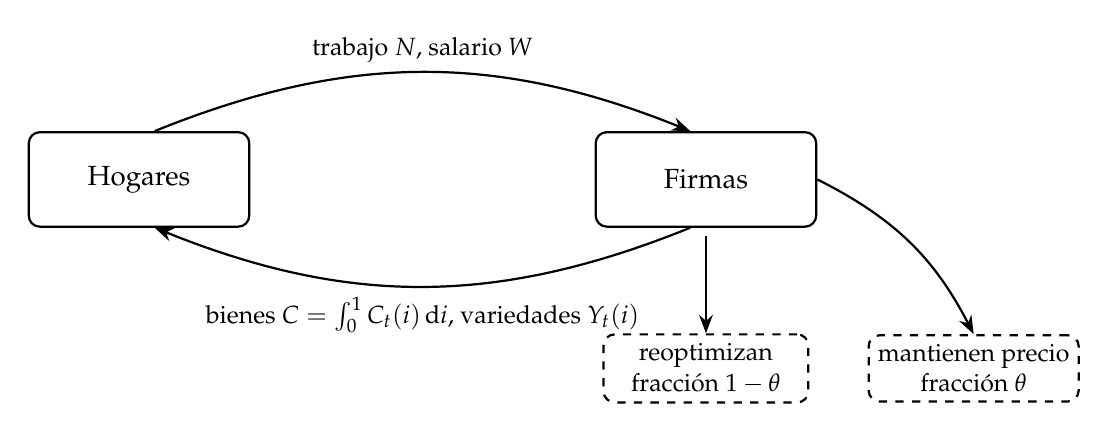
\begin{tikzpicture}[>=Stealth,line width=0.8pt]
  \node[draw,rounded corners,minimum width=2.8cm,minimum height=1.2cm] (H) at (0,0) {Hogares};
  \node[draw,rounded corners,minimum width=2.8cm,minimum height=1.2cm] (F) at (7.2,0) {Firmas};
  \draw[->] (H.north) ++(0.2,0) to[bend left=22] node[above,font=\small]{trabajo $N$, salario $W$} ($(F.north)+(-0.2,0)$);
  \draw[->] ($(F.south)+(-0.2,0)$) to[bend left=22] node[below,font=\small]{bienes $C=\int_{0}^{1}C_{t}(i)\,\mathrm{d}i$, variedades $Y_{t}(i)$} ($(H.south)+(0.2,0)$);
  \node[draw,dashed,rounded corners,align=center,font=\small,minimum width=2.6cm] (R) at (7.2,-2.4) {reoptimizan\\ fracción $1-\theta$};
  \node[draw,dashed,rounded corners,align=center,font=\small,minimum width=2.6cm] (K) at (10.6,-2.4) {mantienen precio\\ fracción $\theta$};
  \draw[->] (F.south) ++(0,-0.1) -- (R.north);
  \draw[->] (F.east) to[bend left=18] (K.north);
\end{tikzpicture}
\caption{Agentes y mercados del modelo NK cerrado. Los hogares ofrecen trabajo y demandan la canasta
de variedades; cada firma fija el precio de su variedad y, bajo Calvo, sólo una fracción $1-\theta$
reoptimiza en cada período.}
\end{figure}

\begin{clave}[La rigidez es lo que da mordida a la demanda]
Con precios rígidos, la política monetaria tiene efectos sobre las asignaciones reales. El modelo NK
trata sobre \emph{mark-ups flexibles}: los mark-ups son variables aleatorias que se mueven según
expectativas, y las firmas son \emph{forward looking}.
\end{clave}

En cada período la firma reoptimiza su precio con probabilidad $1-\theta$ y lo mantiene con
probabilidad $\theta$ (lotería de Calvo):
\begin{equation}
P_{it}=
\begin{cases}
\widetilde{P}_{it}, & \text{con prob.\ }1-\theta\ \ \text{(reoptimiza),}\\[3pt]
P_{it-1}, & \text{con prob.\ }\theta\ \ \text{(mantiene).}
\end{cases}
\end{equation}
La demanda por la variedad y su producción son
\begin{equation}
X_{it}=\Big(\frac{P_{it}}{P_{t}}\Big)^{-\varepsilon}Y_{t},
\qquad Y_{it}=z_{t}h_{it},
\qquad \Pi_{it}=P_{it}X_{it}-W_{t}h_{it}\ \ \text{(beneficio nominal).}
\end{equation}
El \textbf{factor de descuento estocástico nominal} es
$X_{t,t+s}=\beta^{s}\dfrac{\lambda_{t+s}}{\lambda_{t}}\dfrac{P_{t}}{P_{t+s}}$, con $X_{t,t}=1$, y satisface
la propiedad multiplicativa $X_{t,t+1+s}=X_{t,t+1}\,X_{t+1,t+1+s}$, que es la que permite escribir el
problema en forma recursiva. La firma maximiza el valor presente neto de beneficios reales sujeta a la
restricción de producción $z_{t+j}h_{it+j}\ge X_{it+j}$, cuyo multiplicador $MC_{it}$ captura cuánto cae
el valor de la firma si se le demanda una unidad adicional de producto (el costo marginal). El operador
$\E_{t}$ recoge \emph{dos} fuentes de incertidumbre: la agregada y la idiosincrática de la lotería de
Calvo; en adelante se usa para la incertidumbre agregada.

\subsubsection{Problema de la firma que reoptimiza}

Una firma que reoptimiza en $t$ elige $\widetilde{P}_{t}=P_{t}(i)$ sabiendo que su precio seguirá
vigente $k$ períodos con probabilidad $\theta^{k}$. Maximiza el valor presente de sus beneficios
reales:
\begin{equation}
\max_{P_{t}(i)}\ \E_{t}\sum_{k=0}^{\infty}\theta^{k}m_{t+k}\,\frac{\Pi_{t+k}(i)}{P_{t+k}},
\qquad m_{t+k}=\beta^{k}\Big(\frac{C_{t+k}}{C_{t}}\Big)^{-\sigma},
\end{equation}
sujeto a $Y_{t+k}(i)=\big(P_{t}(i)/P_{t+k}\big)^{-\varepsilon}Y_{t+k}$ y $N_{t+k}(i)=Y_{t+k}(i)/A_{t+k}$.
Sustituyendo estas dos restricciones, el beneficio real en $t+k$ de un precio fijado en $t$ es
\begin{align}
\frac{\Pi_{t+k}(i)}{P_{t+k}}
&=\frac{P_{t}(i)}{P_{t+k}}\Big(\frac{P_{t}(i)}{P_{t+k}}\Big)^{-\varepsilon}Y_{t+k}
-\frac{W_{t+k}}{A_{t+k}P_{t+k}}\Big(\frac{P_{t}(i)}{P_{t+k}}\Big)^{-\varepsilon}Y_{t+k} \notag\\[2pt]
&=P_{t}(i)^{1-\varepsilon}P_{t+k}^{\varepsilon-1}Y_{t+k}
-\frac{W_{t+k}}{A_{t+k}}\,P_{t}(i)^{-\varepsilon}P_{t+k}^{\varepsilon-1}Y_{t+k}.
\end{align}

\subsubsection{Condición de primer orden y precio de reoptimización}

Derivando la suma respecto de $P_{t}(i)$,
\begin{equation}
\E_{t}\sum_{k=0}^{\infty}\theta^{k}m_{t+k}\Big[(1-\varepsilon)P_{t}(i)^{-\varepsilon}P_{t+k}^{\varepsilon-1}Y_{t+k}
+\varepsilon\,\frac{W_{t+k}}{A_{t+k}}P_{t}(i)^{-\varepsilon-1}P_{t+k}^{\varepsilon-1}Y_{t+k}\Big]=0 .
\end{equation}
Multiplicando por $P_{t}(i)^{\varepsilon+1}$ y separando ambos términos,
\begin{equation}
(\varepsilon-1)\,P_{t}(i)\,\E_{t}\sum_{k=0}^{\infty}\theta^{k}m_{t+k}\big[P_{t+k}^{\varepsilon-1}Y_{t+k}\big]
=\varepsilon\,\E_{t}\sum_{k=0}^{\infty}\theta^{k}m_{t+k}\Big[\frac{W_{t+k}}{A_{t+k}}P_{t+k}^{\varepsilon-1}Y_{t+k}\Big],
\end{equation}
de donde el \textbf{precio de reoptimización} es
\begin{equation}
\widetilde{P}_{t}=\frac{\varepsilon}{\varepsilon-1}\,
\frac{\E_{t}\sum_{k=0}^{\infty}\theta^{k}m_{t+k}\big[\tfrac{W_{t+k}}{A_{t+k}}P_{t+k}^{\varepsilon-1}Y_{t+k}\big]}
{\E_{t}\sum_{k=0}^{\infty}\theta^{k}m_{t+k}\big[P_{t+k}^{\varepsilon-1}Y_{t+k}\big]}
\qquad\Big(\text{si }\theta=0:\ \widetilde{P}_{t}=\tfrac{\varepsilon}{\varepsilon-1}\mc_{t}\Big).
\end{equation}
En el límite sin rigidez ($\theta=0$) se recupera el \emph{markup} constante sobre el costo marginal.

\subsubsection{Forma recursiva}

Definimos las variables auxiliares $X_{1,t}$ (numerador) y $X_{2,t}$ (denominador). Tomando $X_{1,t}$,
se separa el término $k=0$ y en el resto se hace el cambio de índice $j=k-1$:
\begin{equation}
X_{1,t}=\underbrace{\frac{W_{t}}{A_{t}}P_{t}^{\varepsilon-1}Y_{t}}_{k=0}
+\E_{t}\sum_{j=0}^{\infty}\theta^{\,j+1}m_{t+j+1}\Big[\frac{W_{t+j+1}}{A_{t+j+1}}P_{t+j+1}^{\varepsilon-1}Y_{t+j+1}\Big].
\end{equation}
Usando $m_{t+j+1}=\beta^{\,j+1}\big(\tfrac{C_{t+j+1}}{C_{t}}\big)^{-\sigma}
=\theta^{0}\,\beta\big(\tfrac{C_{t+1}}{C_{t}}\big)^{-\sigma}\cdot\beta^{\,j}\big(\tfrac{C_{t+j+1}}{C_{t+1}}\big)^{-\sigma}$
y factorizando el término común, la suma restante es $\theta\beta\big(\tfrac{C_{t+1}}{C_{t}}\big)^{-\sigma}X_{1,t+1}$.
Lo mismo para $X_{2,t}$, de modo que cada suma se vuelve recursiva:
\begin{align}
X_{1,t}&=\frac{W_{t}}{A_{t}}P_{t}^{\varepsilon-1}Y_{t}
+\theta\beta\,\E_{t}\Big[\big(\tfrac{C_{t+1}}{C_{t}}\big)^{-\sigma}X_{1,t+1}\Big], \\
X_{2,t}&=P_{t}^{\varepsilon-1}Y_{t}
+\theta\beta\,\E_{t}\Big[\big(\tfrac{C_{t+1}}{C_{t}}\big)^{-\sigma}X_{2,t+1}\Big],
\qquad
P_{t}^{\#}=\frac{\widetilde{P}_{t}}{P_{t}}=\frac{\varepsilon}{\varepsilon-1}\frac{X_{1,t}}{X_{2,t}} .
\end{align}
Las empresas están dispuestas a flexibilizar sus mark-ups para hacer un \emph{pricing} óptimo.

\subsubsection{Agregación e ineficiencia}

De $Y_{t}(i)=(P_{t}(i)/P_{t})^{-\varepsilon}Y_{t}$ y $Y_{t}(i)=A_{t}N_{t}(i)$, integrando sobre las
variedades con $\int_{0}^{1}N(i)\dd i=N$,
\begin{equation}
A_{t}\underbrace{\Big[\int_{0}^{1}\big(\tfrac{P(i)}{P_{t}}\big)^{-\varepsilon}\dd i\Big]^{-1}}_{1/\Delta_{t}}N_{t}=Y_{t}
\ \Longrightarrow\
\boxed{\ \widetilde{A}_{t}\,N_{t}=Y_{t}\ },
\qquad
\widetilde{A}_{t}=\frac{A_{t}}{\Delta_{t}},
\end{equation}
donde $\Delta_{t}=\int_{0}^{1}(P(i)/P_{t})^{-\varepsilon}\dd i\ge1$ es la dispersión de precios.
\emph{Con Calvo, la ineficiencia entra a través de la productividad}; con precios flexibles
$\Delta_{t}=1$ y $A_{t}N_{t}=Y_{t}$.

\subsubsection{Evolución de la inflación y dispersión de precios}

\textbf{Índice de precios.} De $P_{t}^{1-\varepsilon}=\int_{0}^{1}P_{it}^{1-\varepsilon}\dd i$, se parte la
integral entre la fracción $\theta$ que mantuvo el precio del período anterior y la fracción $1-\theta$
que reoptimizó a $\widetilde{P}_{t}$:
\begin{equation}
P_{t}^{1-\varepsilon}=\int_{0}^{\theta}P_{it-1}^{1-\varepsilon}\dd i+\int_{0}^{1-\theta}\widetilde{P}_{t}^{1-\varepsilon}\dd i
=\theta\,P_{t-1}^{1-\varepsilon}+(1-\theta)\widetilde{P}_{t}^{1-\varepsilon}.
\end{equation}
Dividiendo por $P_{t}^{1-\varepsilon}$, con $P_{t}^{\#}=\widetilde{P}_{t}/P_{t}$ y $\pi_{t}=P_{t}/P_{t-1}$,
\begin{equation}
1=\theta\Big(\frac{P_{t-1}}{P_{t}}\Big)^{1-\varepsilon}+(1-\theta)\big(P_{t}^{\#}\big)^{1-\varepsilon}
=\theta\,\pi_{t}^{\varepsilon-1}+(1-\theta)\big(P_{t}^{\#}\big)^{1-\varepsilon}.
\end{equation}
\textbf{Dispersión de precios.} Análogamente, partiendo
$\Delta_{t}=\int_{0}^{1}(P_{it}/P_{t})^{-\varepsilon}\dd i$ y usando
$(P_{it-1}/P_{t})^{-\varepsilon}=(P_{it-1}/P_{t-1})^{-\varepsilon}\pi_{t}^{\varepsilon}$ en el grupo que no ajusta,
\begin{equation}
\Delta_{t}=\theta\,\pi_{t}^{\varepsilon}\!\int_{0}^{\theta}\Big(\frac{P_{it-1}}{P_{t-1}}\Big)^{-\varepsilon}\dd i
+(1-\theta)\big(P_{t}^{\#}\big)^{-\varepsilon}
=\theta\,\pi_{t}^{\varepsilon}\Delta_{t-1}+(1-\theta)\big(P_{t}^{\#}\big)^{-\varepsilon},
\end{equation}
con $\Delta_{t}\ge1$ (si $\Delta_{t}>1$ la dispersión de precios es ineficiente).
Loglinealizamos alrededor de un estado estacionario no estocástico
($\widetilde{X}_{t}=\ln X_{t}-\ln X$, $X_{t}\approx X(1+\widetilde{X}_{t})$), de donde
$\widetilde{P}_{t}^{\#}=\dfrac{\theta}{1-\theta}\widetilde{\pi}_{t}$. Tomando logaritmos en la Euler
$C_{t}^{-\sigma}=\beta\E_{t}[(P_{t}/P_{t+1})(1+i_{t+1})C_{t+1}^{-\sigma}]$,
\begin{equation}
-\sigma\ln C_{t}=\ln\beta-\E_{t}\pi_{t+1}+\ln(1+i_{t})-\sigma\ln C_{t+1},
\end{equation}
y restando el estado estacionario término a término se obtiene
$-\sigma\widetilde{C}_{t}=-\sigma\E_{t}\widetilde{C}_{t+1}+\widetilde{i}_{t}-\E_{t}\widetilde{\pi}_{t+1}$.
Expresando todo en \emph{brechas} respecto del equilibrio eficiente sin rigideces
($\widetilde{y}_{t}^{\,n}=\E_{t}\widetilde{y}_{t+1}^{\,n}-\tfrac{1}{\sigma}r_{t}^{n}$) y restando, se
llega a la IS dinámica en brechas:
\begin{equation}
\boxed{\ \widetilde{x}_{t}=\E_{t}\widetilde{x}_{t+1}-\frac{1}{\sigma}\big(\widetilde{i}_{t}-\E_{t}\widetilde{\pi}_{t+1}-\widetilde{r}_{t}^{\,n}\big)\ },
\qquad
\widetilde{x}_{t}\equiv\widetilde{Y}_{t}-\widetilde{y}_{t}^{\,n}.
\end{equation}
La curva de Phillips NK de Calvo resultante es
\begin{equation}
\widehat{\pi}_{t}=\beta\,\E_{t}\widehat{\pi}_{t+1}+\kappa\,\widehat{\mc}_{t},
\qquad
\kappa=\frac{(1-\theta)(1-\beta\theta)}{\theta}.
\end{equation}

\paragraph{Sistema completo de Calvo.} De forma equivalente, con las variables recursivas
$f^{1}_{t},f^{2}_{t}$ (numerador y denominador del precio de reoptimización), la evolución de la inflación queda caracterizada por
\begin{align}
f^{1}_{t}&=\big(P_{t}^{\#}\big)^{1-\varepsilon}Y_{t}\,\frac{\varepsilon-1}{\varepsilon}
+\theta\,\E_{t}\Big\{X_{t,t+1}\big(P_{t}^{\#}/P_{t+1}^{\#}\big)^{1-\varepsilon}\pi_{t+1}^{\varepsilon}\,f^{1}_{t+1}\Big\},\\
f^{2}_{t}&=\big(P_{t}^{\#}\big)^{-\varepsilon}Y_{t}\,\mc_{t}
+\theta\,\E_{t}\Big\{X_{t,t+1}\big(P_{t}^{\#}/P_{t+1}^{\#}\big)^{-\varepsilon}\pi_{t+1}^{\varepsilon+1}\,f^{2}_{t+1}\Big\},\\
f^{1}_{t}&=f^{2}_{t},\qquad
1=\theta\,\pi_{t}^{\varepsilon-1}+(1-\theta)\big(P_{t}^{\#}\big)^{1-\varepsilon},\qquad
\Delta_{t}=\theta\,\pi_{t}^{\varepsilon}\Delta_{t-1}+(1-\theta)\big(P_{t}^{\#}\big)^{-\varepsilon}.
\end{align}
La separación entre el término $k=0$ y el resto (con el cambio de índice $s=j-1$, la propiedad
$X_{t,t+1+s}=X_{t,t+1}X_{t+1,t+1+s}$ y la ley de expectativas iteradas) es lo que convierte las sumas
infinitas en estas recursiones.

\subsection{Intuición del modelo neokeynesiano}

\textbf{Ley de los grandes números.} Como Calvo es una lotería (un proceso de Poisson de
reoptimización), la fracción de firmas que reajusta su precio cada período es \emph{exactamente}
$1-\theta$. Esto permite derivar un índice de precios recursivo y \emph{determinístico} ---y con él la
curva de Phillips--- sin arrastrar la incertidumbre del proceso de reajuste individual de cada firma.

\textbf{Estructura del bien final y las variedades.} El bien final es competitivo y combina un continuo
de variedades, $Y_{t}=\big(\int_{0}^{1}Y_{it}^{\frac{\varepsilon-1}{\varepsilon}}\dd i\big)^{\frac{\varepsilon}{\varepsilon-1}}$
(una canasta agregada). Los bienes intermedios los producen firmas monopolistas: cada firma $i$ produce
su variedad diferenciada, tiene poder de mercado y fija su precio a lo Calvo. La demanda que enfrenta
es $Y_{it}=Y_{t}(P_{it}/P_{t})^{-\varepsilon}$; la variedad es lo que permite la diferenciación (si
todas produjeran el mismo bien, la demanda sería perfectamente elástica y nadie podría cobrar un
\emph{markup}).

\textbf{Asignación eficiente y distorsiones.} La asignación eficiente resuelve el problema del
planificador social que maximiza el bienestar del hogar dadas tecnología y preferencias; en el
equilibrio simétrico ($C_{t}(i)=C_{t}$, $N_{t}(i)=N_{t}$) iguala la tasa marginal de sustitución a la
productividad marginal del trabajo, $-U_{N,t}/U_{C,t}=MPN_{t}=(1-\alpha)A_{t}N_{t}^{-\alpha}$. El modelo
NK básico tiene dos fuentes de distorsión. La primera \emph{no} está ligada a los precios rígidos: es
el \textbf{poder de mercado} de la competencia monopolística, que existe incluso con precios flexibles.
La firma fija el precio con un \emph{markup} sobre el costo marginal,
\begin{equation}
P_{t}=\mathcal{M}\,\frac{W_{t}}{MPN_{t}},\qquad \mathcal{M}=\frac{\varepsilon}{\varepsilon-1}>1,
\end{equation}
de modo que $-U_{N,t}/U_{C,t}=W_{t}/P_{t}=MPN_{t}/\mathcal{M}<MPN_{t}$: el \emph{markup} separa la
asignación de mercado del óptimo, distorsionando a la baja el empleo y el producto.

\textbf{La curva de Phillips NK: intuición.} Con rigideces nominales y competencia monopolística las
empresas cubren el exceso de demanda, de modo que
\[
\uparrow\text{demanda}\ \Rightarrow\ \uparrow\text{producción (ineficiente)}\ \Rightarrow\ \uparrow\text{costo marginal}\ \Rightarrow\ \uparrow\text{inflación.}
\]
Bajo Calvo, las firmas que sí pueden reoptimizar \emph{sobrerreaccionan} (fijan un precio más alto)
porque saben que quizá no podrán ajustar en los próximos períodos; esto aumenta la dispersión de
precios y genera pérdida de bienestar. Cuando se introducen rigideces nominales, los choques reales
tienen efectos sobre la \emph{demanda agregada}: con precios flexibles los mercados se ajustan solos y
se vende todo lo producido; con rigideces, los precios no bajan lo suficiente, quedan demasiado altos
para el nivel de demanda, y las empresas ajustan cantidades ---producción, demanda de trabajo,
salarios.

\textbf{Análisis de choques de productividad.} La tasa de interés natural depende de la
\emph{persistencia} del choque, $r_{t}^{n}=\tfrac{1}{\sigma}\E_{t}\Delta z_{t+1}$. Un choque
\emph{permanente} ($\rho=0.97$) tiene $\E_{t}\Delta z_{t+1}>0$: productividad alta hoy implica alta
mañana, sube el ingreso permanente, y aumentan consumo, producción, empleo y producto. Un choque
\emph{transitorio} ($\rho=0.25$) tiene $\E_{t}\Delta z_{t+1}<0$ (si hoy sube mucho, mañana vuelve a la
media): el ingreso permanente casi no cambia, predomina el efecto ingreso, se produce lo mismo con
menos trabajo, el producto sube poco y la tasa natural \emph{baja} (la economía desea menos ahorro).

\begin{notabox}[Propiedad Fisheriana y anti-Fisheriana]
La \emph{propiedad Fisheriana} dice que cambios \emph{permanentes} de política monetaria mueven la
inflación y la tasa nominal uno a uno. La \emph{anti-Fisheriana}, que cambios \emph{transitorios}
mueven la tasa nominal y la inflación en sentidos \emph{opuestos}. El modelo NK cumple la
anti-Fisheriana por la siguiente cadena: (1)~las firmas fijan precios según costos marginales
esperados; (2)~como el choque es transitorio, la inflación responde poco a una caída de la tasa
nominal; (3)~la tasa real cae; (4)~por sustitución intertemporal sube el consumo presente y con él el
ingreso laboral; (5)~se refuerzan consumo y empleo; (6)~el mayor empleo eleva costos marginales y
salarios; (7)~la inflación sube. Cumple además la Fisheriana, porque hereda las propiedades de largo
plazo del modelo RBC.
\end{notabox}

\textbf{Rigideces nominales y el modelo de Christiano--Eichenbaum--Evans.} Las fricciones a lo Calvo
tienen sentido con inflación moderada; su virtud es capturar que, en ese régimen, las firmas responden
a variaciones de demanda ajustando \emph{cantidades} y no precios. Para que esto sea plausible se
necesitan costos marginales \emph{acíclicos} (así las firmas satisfacen la demanda y se amortiguan los
movimientos de la inflación), lo que suele requerir \emph{salarios rígidos}. El modelo NK empírico de
Christiano, Eichenbaum y Evans añade dos ingredientes para replicar las respuestas \emph{hump-shaped}
de los VAR: \emph{hábitos de consumo} en la utilidad (suavizan la respuesta del consumo, que con
utilidad separable sería demasiado abrupta) y \emph{costos de ajuste de la inversión} (dan a la
inversión una respuesta gradual como en las funciones de impulso-respuesta estimadas).

\section{El modelo NK a lo Rotemberg}

Una alternativa a Calvo modela el costo de reajustar precios como un costo cuadrático (Rotemberg), en lugar de una lotería de reoptimización.

\subsection{Rigideces a la Rotemberg (costos de ajuste cuadráticos)}

Con competencia monopolística y hogar con dinero en la utilidad, los productores de bienes finales
usan la tecnología Dixit--Stiglitz
$Y_{t}=\big(\int_{0}^{1}x_{it}^{\frac{\varepsilon-1}{\varepsilon}}\dd i\big)^{\frac{\varepsilon}{\varepsilon-1}}$,
de donde la demanda por el insumo intermedio y el índice de precios son
\begin{equation}
x_{it}=\Big(\frac{P_{it}}{P_{t}}\Big)^{-\varepsilon}Y_{t},
\qquad\qquad
P_{t}=\Big(\int_{0}^{1}P_{it}^{1-\varepsilon}\dd i\Big)^{\frac{1}{1-\varepsilon}} .
\end{equation}
La producción intermedia es $Y_{it}=z_{t}h_{it}$ (productividad agregada). El \textbf{costo de ajuste
de precios} (Rotemberg) es $\dfrac{\phi}{2}\big(\tfrac{P_{it}}{P_{it-1}}-1\big)^{2}P_{i}Y_{t}$: es
costoso cambiar precios bruscamente. Una vez puesto el precio, se produce para satisfacer la demanda
($Y_{it}\ge x_{it}$). El lagrangiano para elegir $P_{it}$ y $h_{it}$ es
\begin{equation}
\E_{0}\Big\{\sum_{s\ge0}X_{t,t+s}\Big[P_{it}\Big(\tfrac{P_{it}}{P_{t}}\Big)^{-\varepsilon}Y_{t}
-W_{t}h_{it}-\tfrac{\phi}{2}\big(\tfrac{P_{t}}{P_{t-1}}-1\big)^{2}P_{t}Y_{t}
+MC_{it}\big(z_{t}h_{it}-\big(\tfrac{P_{it}}{P_{t}}\big)^{-\varepsilon}Y_{t}\big)\Big]\Big\},
\end{equation}
con el \textbf{SDF nominal} $X_{t,t+s}=\beta^{s}\dfrac{\lambda_{t+s}}{\lambda_{t}}\dfrac{P_{t}}{P_{t+s}}$.
La CPO de $h_{it}$ da $MC_{t}=W_{t}/z_{t}$ (todas las firmas enfrentan el mismo costo marginal). La CPO
de $P_{it}$, reescribiendo el lagrangiano en términos de $P_{it}/P_{t}$ y derivando, es
\begin{align}
&\Big[(1-\varepsilon)\tfrac{1}{P_{t}}\big(\tfrac{P_{it}}{P_{t}}\big)^{-\varepsilon}
+\varepsilon\tfrac{MC_{t}}{P_{t}}\big(\tfrac{P_{it}}{P_{t}}\big)^{-\varepsilon-1}\tfrac{1}{P_{t}}
-\phi\big(\tfrac{P_{it}}{P_{it-1}}-1\big)\tfrac{1}{P_{it-1}}\Big]P_{t}Y_{t} \notag\\
&\qquad\qquad
+\E_{t}\Big\{X_{t,t+1}\phi\big(\tfrac{P_{it+1}}{P_{it}}-1\big)\tfrac{P_{it+1}}{P_{it}^{2}}P_{t+1}Y_{t+1}\Big\}=0 .
\end{align}
Si $\phi=0$ se reduce a $P_{it}=\tfrac{\varepsilon}{\varepsilon-1}MC_{t}$. Como todas las firmas
enfrentan el mismo problema, en el \textbf{equilibrio simétrico} $P_{it}=P_{t}$; con $\mc_{t}=MC_{t}/P_{t}$
la CPO se simplifica a la \textbf{curva de Phillips NK no lineal}:
\begin{equation}
\boxed{\ \varepsilon-1=\mc_{t}\,\varepsilon-\phi(\pi_{t}-1)\pi_{t}
+\beta\phi\,\E_{t}\Big\{\frac{\lambda_{t+1}}{\lambda_{t}}\frac{Y_{t+1}}{Y_{t}}(\pi_{t+1}-1)\pi_{t+1}\Big\}\ }.
\end{equation}
El mercado de trabajo agrega $h_{t}=\int_{0}^{1}h_{it}\dd i$; el costo de ajuste está denominado en
bienes finales, de modo que el mercado de bienes se limpia como
\begin{equation}
C_{t}+\frac{\phi}{2}(\pi_{t}-1)^{2}Y_{t}=Y_{t}
\ \Longrightarrow\
C_{t}=Y_{t}\Big[1-\frac{\phi}{2}(\pi_{t}-1)^{2}\Big].
\end{equation}
Estas condiciones, con $\mc_{t}z_{t}=W_{t}$, las del hogar
($U_{C_{t}}=\lambda_{t}$, $1=R_{t}\E_{t}\{\beta\tfrac{\lambda_{t+1}}{\lambda_{t}}\tfrac{1}{\pi_{t+1}}\}$,
$-U_{N_{t}}/U_{C_{t}}=W_{t}$, $\lambda_{t}=U_{M_{t}}+\beta\E_{t}\{\lambda_{t+1}/\pi_{t+1}\}$) y el
\emph{market clearing} $z_{t}h_{t}=Y_{t}$ cierran el modelo en las variables
$\{Y_{t},\pi_{t},C_{t},\lambda_{t},h_{t},M_{t},W_{t},\mc_{t},R_{t},z_{t}\}$.

\subsection{La curva de Phillips NK (loglinealización)}

Se loglineariza la curva de Phillips no lineal alrededor del estado estacionario de inflación cero
($\pi=1$, $\mc=\tfrac{\varepsilon-1}{\varepsilon}$). El término $\phi(\pi_{t}-1)\pi_{t}$ se linealiza con
$\tfrac{\dd}{\dd\pi}[(\pi-1)\pi]\big|_{\pi=1}=2\pi-1\big|_{\pi=1}=1$ y $\pi_{t}-1\approx\widehat{\pi}_{t}$,
de modo que $\phi(\pi_{t}-1)\pi_{t}\approx\phi\,\widehat{\pi}_{t}$; el término adelantado
$\beta\phi\,\E_{t}\{(\pi_{t+1}-1)\pi_{t+1}\}\approx\beta\phi\,\E_{t}\widehat{\pi}_{t+1}$ (los cocientes
$\lambda_{t+1}/\lambda_{t}$ y $Y_{t+1}/Y_{t}$ valen $1$ a primer orden); y $\mc_{t}\varepsilon\approx
(\varepsilon-1)(1+\widehat{\mc}_{t})$. Sustituyendo en $\varepsilon-1=\mc_{t}\varepsilon-\phi(\pi_{t}-1)\pi_{t}+\beta\phi\E_{t}\{\cdots\}$,
\begin{equation}
\varepsilon-1=(\varepsilon-1)+(\varepsilon-1)\widehat{\mc}_{t}-\phi\,\widehat{\pi}_{t}+\beta\phi\,\E_{t}\widehat{\pi}_{t+1}
\ \Longrightarrow\
\phi\,\widehat{\pi}_{t}=(\varepsilon-1)\widehat{\mc}_{t}+\beta\phi\,\E_{t}\widehat{\pi}_{t+1},
\end{equation}
y dividiendo por $\phi$ se obtiene la \textbf{curva de Phillips NK}:
\begin{equation}
\widehat{\pi}_{t}=\kappa\,\widehat{\mc}_{t}+\beta\,\E_{t}\widehat{\pi}_{t+1},
\qquad
\kappa=\frac{\varepsilon-1}{\phi}\quad(\text{Rotemberg}).
\end{equation}
Si $\phi\to\infty$, entonces $\kappa\to0$ y $\widehat{\pi}_{t}=0$ (precios rígidos). Iterando hacia
adelante y sustituyendo repetidamente $\E_{t}\widehat{\pi}_{t+1}$,
\begin{align}
\widehat{\pi}_{t}&=\kappa\,\widehat{\mc}_{t}+\beta\E_{t}\big[\kappa\widehat{\mc}_{t+1}+\beta\E_{t+1}\widehat{\pi}_{t+2}\big] \notag\\
&=\kappa\,\widehat{\mc}_{t}+\beta\E_{t}\big[\kappa\widehat{\mc}_{t+1}+\beta\E_{t+1}[\kappa\widehat{\mc}_{t+2}+\beta\E_{t+2}\widehat{\pi}_{t+3}]\big] \notag\\
&=\kappa\,\widehat{\mc}_{t}+\kappa\beta\E_{t}\widehat{\mc}_{t+1}+\kappa\beta^{2}\E_{t}\widehat{\mc}_{t+2}+\beta^{3}\E_{t}\widehat{\pi}_{t+3}
=\dots \notag\\
&=\kappa\sum_{j=0}^{\infty}\beta^{j}\,\E_{t}\{\widehat{\mc}_{t+j}\}
\qquad\Big(\lim_{s\to\infty}\beta^{s}\E_{t}\widehat{\pi}_{t+s}=0\Big):
\end{align}
La inflación es \emph{forward looking}: depende de los costos marginales futuros esperados.

\subsubsection{Mecanismo de transmisión}

Con
$u\big(C_{t},h_{t},\tfrac{M_{t}}{P_{t}}\big)
=\dfrac{C_{t}^{1-\sigma}}{1-\sigma}-\chi\dfrac{h_{t}^{1+\varphi}}{1+\varphi}
+\xi\dfrac{(M_{t}/P_{t})^{1-\nu}}{1-\nu}$,
la Euler $C_{t}^{-\sigma}=R_{t}\E_{t}\{\beta C_{t+1}^{-\sigma}/\pi_{t+1}\}$ loglinealiza a la
\textbf{IS dinámica}:
\begin{equation}
\boxed{\ \widehat{C}_{t}=\E_{t}\widehat{C}_{t+1}-\sigma^{-1}\big(\widehat{R}_{t}-\E_{t}\widehat{\pi}_{t+1}\big)\ }
\ \Longrightarrow\
\widehat{C}_{t}=-\sigma^{-1}\sum_{j=0}^{\infty}\big(\widehat{R}_{t+j}-\E_{t}\widehat{\pi}_{t+1+j}\big):
\end{equation}
El consumo es \emph{forward looking}.

\begin{notabox}[Neutralidad del dinero y anclaje de expectativas]
Si los precios son flexibles, un cambio en política monetaria genera cambios en los precios (vía
cambios en el consumo) y mueve las curvas de oferta y demanda sin que suceda nada con el consumo
real: cuando los cambios en la tasa real son compensados por cambios en la inflación esperada, el
consumo no se mueve. Las rigideces de precios rompen esto; depende de la habilidad de la política
monetaria de anclar las expectativas de inflación. Importa la trayectoria futura de tasas (la
\emph{yield curve} $\sum_{j\ge0}\widehat{R}_{t+j}$). El parámetro clave es $1/\sigma$ (EIS): mientras
más baja la EIS, mayor el cambio requerido en $\widehat{R}_{t+j}-\E_{t}\{\widehat{\pi}\}$ para producir
un cambio en el consumo. Si la \emph{yield curve} se aplana ($\downarrow\sum\widehat{R}$), sube el
consumo agregado.
\end{notabox}

\begin{figure}[h]
\centering
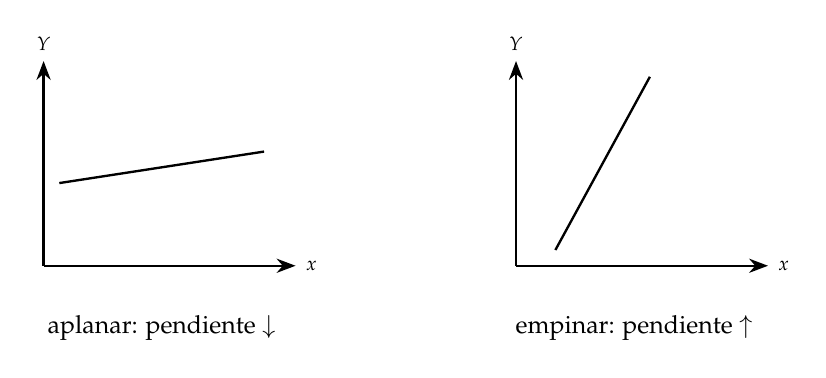
\begin{tikzpicture}[>=Stealth,line width=0.85pt]
  \begin{scope}
    \draw[->](0,0)--(3.2,0) node[right]{\scriptsize $x$};
    \draw[->](0,0)--(0,2.6) node[above]{\scriptsize $Y$};
    \draw (0.2,1.05)--(2.8,1.45);
    \node[below] at (1.5,-0.5){\small aplanar: pendiente $\downarrow$};
  \end{scope}
  \begin{scope}[xshift=6cm]
    \draw[->](0,0)--(3.2,0) node[right]{\scriptsize $x$};
    \draw[->](0,0)--(0,2.6) node[above]{\scriptsize $Y$};
    \draw (0.5,0.2)--(1.7,2.4);
    \node[below] at (1.5,-0.5){\small empinar: pendiente $\uparrow$};
  \end{scope}
\end{tikzpicture}
\caption{Aplanar reduce la pendiente y empinar la aumenta. Si la \emph{yield curve} se aplana
($\downarrow\sum_{j}\widehat{R}_{t+j}$), sube el consumo agregado.}
\end{figure}

\section{Calvo Pricing: otra forma de ver las rigideces}

Vista junto a Rotemberg, la fijación de precios a lo Calvo es la forma \emph{microfundada} de la misma
rigidez nominal: en vez de un costo de ajuste \emph{ad hoc}, una fracción $1-\theta$ de firmas
reoptimiza cada período. La derivamos de nuevo, ahora con la notación $f^{1}_{t},f^{2}_{t}$ del
manuscrito (complementaria a la de $X_{1,t},X_{2,t}$ usada antes), separando de forma \emph{explícita}
el término $j=0$.

\subsection{Planteamiento y condiciones de primer orden}

Con demanda $X_{it}=(P_{it}/P_{t})^{-\varepsilon}Y_{t}$, producción $Y_{it}=z_{t}h_{it}$ y lotería de
Calvo ($P_{it}=\widetilde{P}_{it}$ con prob.\ $1-\theta$, o $P_{it-1}$ con prob.\ $\theta$), el
beneficio nominal es $\Pi_{it}=P_{it}X_{it}-W_{t}h_{it}$. El factor de descuento nominal
$X_{t,t+s}=\beta^{s}\tfrac{\lambda_{t+s}}{\lambda_{t}}\tfrac{P_{t}}{P_{t+s}}$ cumple $X_{t,t}=1$ y
$X_{t,t+s}=X_{t,t+1}X_{t+1,t+2}\cdots X_{t+s-1,t+s}$. La firma que reoptimiza en $t$ elige
$\widetilde{P}_{t}$ y $\{h_{it+j}\}$ para maximizar el valor presente de beneficios reales, sujeta a la
restricción de producción $z_{t+j}h_{it+j}\ge X_{it+j}$ con multiplicador $MC_{it+j}$:
\begin{equation}
\E_{t}\sum_{j=0}^{\infty}\theta^{j}X_{t,t+j}\Big[P_{it+j}X_{it+j}-W_{t+j}h_{it+j}
+MC_{it+j}\big(z_{t+j}h_{it+j}-X_{it+j}\big)\Big].
\end{equation}
El operador $\E_{t}$ recoge dos fuentes de incertidumbre (agregada e idiosincrática de la lotería). La
CPO de $h_{it+j}$ da $W_{t+j}=MC_{it+j}z_{t+j}$, es decir $\mc_{t}=w_{t}/z_{t}$ (costo marginal real,
común a todas las firmas). Escribiendo el beneficio real de un precio $\widetilde{P}_{t}$ vigente en
$t+j$ como $(\widetilde{P}_{t}/P_{t+j})^{1-\varepsilon}Y_{t+j}-\mc_{t+j}(\widetilde{P}_{t}/P_{t+j})^{-\varepsilon}Y_{t+j}$,
la CPO $\partial/\partial\widetilde{P}_{t}=0$ da la condición de reoptimización $\ f^{1}_{t}=f^{2}_{t}$,
con
\begin{align}
f^{1}_{t}&=\E_{t}\sum_{j=0}^{\infty}\theta^{j}X_{t,t+j}\,\frac{\varepsilon-1}{\varepsilon}\Big(\frac{\widetilde{P}_{t}}{P_{t+j}}\Big)^{1-\varepsilon}Y_{t+j},\\
f^{2}_{t}&=\E_{t}\sum_{j=0}^{\infty}\theta^{j}X_{t,t+j}\,\mc_{t+j}\Big(\frac{\widetilde{P}_{t}}{P_{t+j}}\Big)^{-\varepsilon}Y_{t+j}.
\end{align}

\subsection{Forma recursiva: se separa el término \texorpdfstring{$j=0$}{j=0}}

Tomamos $f^{1}_{t}$ y escribimos aparte el sumando $j=0$ (para el cual $\theta^{0}=1$, $X_{t,t}=1$,
$P_{t+0}=P_{t}$, $Y_{t+0}=Y_{t}$) del resto de la suma:
\begin{equation}
f^{1}_{t}=\underbrace{\frac{\varepsilon-1}{\varepsilon}\Big(\frac{\widetilde{P}_{t}}{P_{t}}\Big)^{1-\varepsilon}Y_{t}}_{j=0}
+\E_{t}\sum_{j=1}^{\infty}\theta^{j}X_{t,t+j}\,\frac{\varepsilon-1}{\varepsilon}\Big(\frac{\widetilde{P}_{t}}{P_{t+j}}\Big)^{1-\varepsilon}Y_{t+j}.
\end{equation}
En la suma restante se hace el cambio de índice $s=j-1$ (de modo que $j=1\Rightarrow s=0$) y se usa la
propiedad multiplicativa $X_{t,t+1+s}=X_{t,t+1}\,X_{t+1,t+1+s}$:
\begin{equation}
f^{1}_{t}=\frac{\varepsilon-1}{\varepsilon}\Big(\frac{\widetilde{P}_{t}}{P_{t}}\Big)^{1-\varepsilon}Y_{t}
+\theta\,\E_{t}\Big\{X_{t,t+1}\!\sum_{s=0}^{\infty}\theta^{s}X_{t+1,t+1+s}\,\frac{\varepsilon-1}{\varepsilon}\Big(\frac{\widetilde{P}_{t}}{P_{t+1+s}}\Big)^{1-\varepsilon}Y_{t+1+s}\Big\}.
\end{equation}
Separando $\big(\tfrac{\widetilde{P}_{t}}{P_{t+1+s}}\big)^{1-\varepsilon}
=\big(\tfrac{\widetilde{P}_{t}}{\widetilde{P}_{t+1}}\big)^{1-\varepsilon}\big(\tfrac{\widetilde{P}_{t+1}}{P_{t+1+s}}\big)^{1-\varepsilon}$
y aplicando la \emph{ley de expectativas iteradas}, el corchete interior es exactamente $f^{1}_{t+1}$.
En términos del precio relativo $P_{t}^{\#}=\widetilde{P}_{t}/P_{t}$ y de $\pi_{t}=P_{t}/P_{t-1}$,
\begin{equation}
f^{1}_{t}=\frac{\varepsilon-1}{\varepsilon}\big(P_{t}^{\#}\big)^{1-\varepsilon}Y_{t}
+\theta\,\E_{t}\Big\{X_{t,t+1}\big(P_{t}^{\#}/P_{t+1}^{\#}\big)^{1-\varepsilon}\pi_{t+1}^{\varepsilon}\,f^{1}_{t+1}\Big\}.
\end{equation}
De forma idéntica (con $-\varepsilon$ en lugar de $1-\varepsilon$ y una potencia extra de $\pi$),
\begin{equation}
f^{2}_{t}=\big(P_{t}^{\#}\big)^{-\varepsilon}Y_{t}\,\mc_{t}
+\theta\,\E_{t}\Big\{X_{t,t+1}\big(P_{t}^{\#}/P_{t+1}^{\#}\big)^{-\varepsilon}\pi_{t+1}^{\varepsilon+1}\,f^{2}_{t+1}\Big\}.
\end{equation}

\subsection{Sistema que caracteriza la inflación}

La reoptimización es $f^{1}_{t}=f^{2}_{t}$. El índice de precios y la dispersión salen de partir la
integral $\int_{0}^{1}=\theta\int_{0}^{\theta}+(1-\theta)\int_{0}^{1-\theta}$ entre las firmas que no
ajustan y las que sí (igual que antes). El sistema completo es
\begin{align}
f^{1}_{t}&=\frac{\varepsilon-1}{\varepsilon}\big(P_{t}^{\#}\big)^{1-\varepsilon}Y_{t}
+\theta\,\E_{t}\big\{X_{t,t+1}\big(P_{t}^{\#}/P_{t+1}^{\#}\big)^{1-\varepsilon}\pi_{t+1}^{\varepsilon}f^{1}_{t+1}\big\},\\
f^{2}_{t}&=\big(P_{t}^{\#}\big)^{-\varepsilon}Y_{t}\,\mc_{t}
+\theta\,\E_{t}\big\{X_{t,t+1}\big(P_{t}^{\#}/P_{t+1}^{\#}\big)^{-\varepsilon}\pi_{t+1}^{\varepsilon+1}f^{2}_{t+1}\big\},\\
f^{1}_{t}&=f^{2}_{t},\qquad
1=\theta\,\pi_{t}^{\varepsilon-1}+(1-\theta)\big(P_{t}^{\#}\big)^{1-\varepsilon},\qquad
\Delta_{t}=\theta\,\pi_{t}^{\varepsilon}\Delta_{t-1}+(1-\theta)\big(P_{t}^{\#}\big)^{-\varepsilon}.
\end{align}
Es el mismo contenido económico que la formulación $X_{1,t}/X_{2,t}$ de la sección anterior; la
diferencia es sólo de normalización.

\begin{notabox}[¿Calvo o Rotemberg?]
El parámetro $\theta$ de Calvo puede estimarse con microdata de precios; $\phi$ de Rotemberg no es
observable. Las similitudes en las curvas de Phillips que producen se deben a que en ambas fricciones
se loglinealiza alrededor de $\pi=0$. En general, hacer Rotemberg equivale a hacer Calvo de manera
indirecta; Rotemberg es más robusto a no linealidades.
\end{notabox}

\subsection{Oferta y demanda agregada en el modelo NK}

En el espacio $(\tilde{x},\pi)$ ---brecha del producto contra inflación--- el modelo se resume en dos
curvas cuyo cruce determina el equilibrio.

\textbf{Oferta agregada (OA).} Es la curva de Phillips,
$\pi_{t}=\beta\,\E_{t}\pi_{t+1}+\kappa\,x_{t}$. Tiene \emph{pendiente positiva}: más brecha positiva
presiona los costos marginales y sube la inflación.

\textbf{Demanda agregada (DA).} No es la IS sola: la IS relaciona la brecha con la \emph{tasa real},
no con la inflación. Para obtener una relación negativa entre $\pi$ y $\tilde{x}$ hay que \emph{cerrar
con la regla de Taylor}. Cuando $\phi_{\pi}>1$ (principio de Taylor), una $\pi$ más alta hace que el
banco central suba $i$ más que uno a uno, sube la tasa real, cae la demanda vía IS y baja la brecha.
Esa cadena da la \emph{pendiente negativa}. La DA del modelo NK es, entonces, la IS y la regla de
Taylor fundidas en una sola relación.

\begin{figure}[h]
\centering
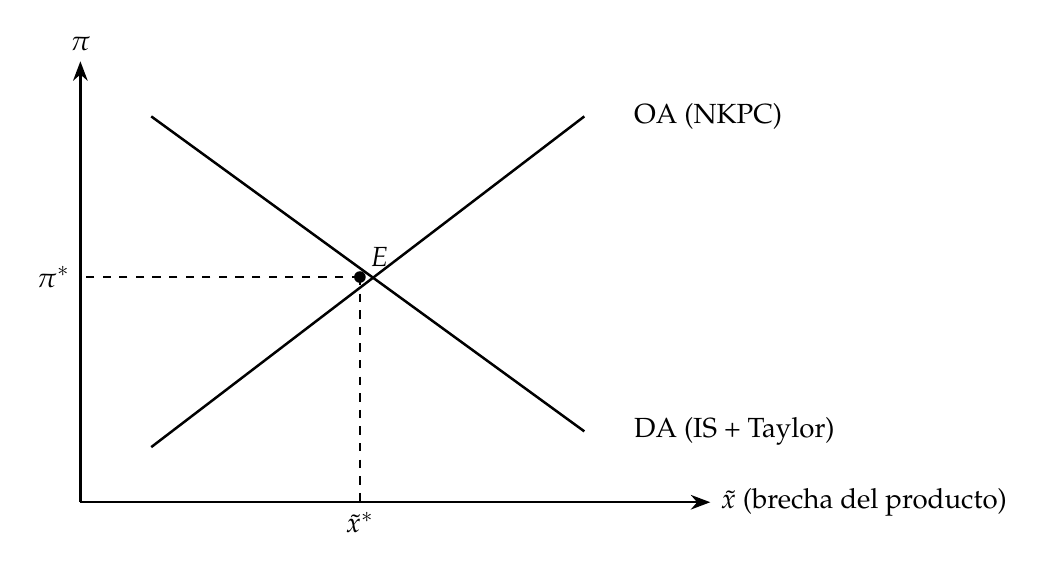
\begin{tikzpicture}[>=Stealth,line width=0.9pt]
  % ejes
  \draw[->] (0,0) -- (8,0) node[right] {$\tilde{x}$ (brecha del producto)};
  \draw[->] (0,0) -- (0,5.6) node[above] {$\pi$};
  % OA: pendiente positiva (curva de Phillips)
  \draw (0.9,0.7) -- (6.4,4.9);
  \node at (6.9,4.9) [right] {OA (NKPC)};
  % DA: pendiente negativa (IS + regla de Taylor)
  \draw (0.9,4.9) -- (6.4,0.9);
  \node at (6.9,0.9) [right] {DA (IS + Taylor)};
  % equilibrio (interseccion aproximada)
  \fill (3.55,2.86) circle (2.1pt);
  \node at (3.55,2.86) [above right] {$E$};
  % guias punteadas
  \draw[dashed] (3.55,2.86) -- (3.55,0) node[below] {$\tilde{x}^{*}$};
  \draw[dashed] (3.55,2.86) -- (0,2.86) node[left] {$\pi^{*}$};
\end{tikzpicture}
\caption{Equilibrio neokeynesiano en el plano $(\tilde{x},\pi)$. La oferta agregada es la curva de
Phillips (NKPC), con pendiente positiva; la demanda agregada combina la IS dinámica con la regla de
Taylor, con pendiente negativa.}
\end{figure}

El equilibrio está en la intersección $E$. Un \emph{choque de demanda} desplaza la DA y el punto se
mueve a lo largo de la OA; un \emph{choque de oferta} desplaza la OA y el punto se mueve a lo largo de
la DA. De ahí el criterio de comovimiento: un choque de demanda mueve producto e inflación en la
\emph{misma} dirección, mientras que un choque de oferta los mueve en direcciones \emph{opuestas}.

\section{Ejercicios: el modelo NK de tres ecuaciones}

El modelo canónico linealizado es
\begin{align}
x_{t}&=\E_{t}x_{t+1}-\big[r_{t}-\E_{t}\pi_{t+1}-r_{t}^{\ast}\big] & &\text{(IS)},\\
r_{t}&=\phi_{\pi}\pi_{t} & &\text{(regla de Taylor)},\\
\pi_{t}&=\beta\,\E_{t}\pi_{t+1}+\kappa\,x_{t}, & r_{t}^{\ast}&=\E_{t}(a_{t+1}-a_{t})\quad\text{(tasa natural)},
\end{align}
con $\kappa=\dfrac{(1-\theta)(1-\beta\theta)(1+\varphi)}{\theta}$.

\subsection{Caso \emph{difference stationary}}

La ley de movimiento en primeras diferencias es $\Delta a_{t}=\rho\,\Delta a_{t-1}+\varepsilon_{t}$, de
modo que $r_{t}^{\ast}=\E_{t}\Delta a_{t+1}=\gamma_{0}\Delta a_{t}$ con $\gamma_{0}=\rho$. Por el método
de \textbf{coeficientes indeterminados}, se conjetura
\begin{equation}
\pi_{t}=\gamma_{1}\Delta a_{t},\qquad x_{t}=\gamma_{2}\Delta a_{t},\qquad r_{t}=\gamma_{3}\Delta a_{t},
\end{equation}
con $\E_{t}x_{t+1}=\rho\gamma_{2}\Delta a_{t}$ y $\E_{t}\pi_{t+1}=\rho\gamma_{1}\Delta a_{t}$.
Reemplazando en la IS,
\begin{equation}
\gamma_{2}\Delta a_{t}=\rho\gamma_{2}\Delta a_{t}-\big(\gamma_{3}\Delta a_{t}-\rho\gamma_{1}\Delta a_{t}-\rho\Delta a_{t}\big),
\end{equation}
y dividiendo entre $\Delta a_{t}$ se obtienen las tres relaciones
\begin{align}
\gamma_{2}&=\rho\gamma_{2}-\gamma_{3}+\gamma_{1}+\rho, &
\gamma_{3}&=\phi_{\pi}\gamma_{1}, &
\gamma_{1}&=\beta\rho\gamma_{1}+\kappa\gamma_{2} .
\end{align}
Definimos la tasa de interés real $\widetilde{r}_{t}=r_{t}-\E_{t}\pi_{t+1}=(\gamma_{3}-\rho\gamma_{1})\Delta a_{t}=\gamma_{4}\Delta a_{t}$.
De la segunda relación, $\gamma_{1}=\gamma_{3}/\phi_{\pi}$; de la tercera,
$(1-\beta\rho)\gamma_{1}=\kappa\gamma_{2}\Rightarrow\gamma_{2}=\tfrac{1-\beta\rho}{\kappa}\tfrac{\gamma_{3}}{\phi_{\pi}}$.
Sustituyendo en la primera reescrita como $(1-\rho)\gamma_{2}+\gamma_{3}-\rho\gamma_{1}=\rho$ y
factorizando $\gamma_{3}$,
\begin{equation}
\gamma_{3}\Big[\frac{(1-\beta\rho)(1-\rho)}{\kappa}\frac{1}{\phi_{\pi}}+1-\frac{\rho}{\phi_{\pi}}\Big]=\rho,
\qquad
\gamma_{4}=\gamma_{3}-\rho\gamma_{1}=\Big(1-\frac{\rho}{\phi_{\pi}}\Big)\gamma_{3},
\end{equation}
de donde la respuesta relativa de la tasa real a la natural es
\begin{equation}
\boxed{\ \Psi=\frac{\widetilde{r}_{t}}{r_{t}^{\ast}}=\frac{\gamma_{4}}{\gamma_{0}}
=\frac{1-\rho/\phi_{\pi}}{\ \dfrac{(1-\beta\rho)(1-\rho)}{\kappa}\dfrac{1}{\phi_{\pi}}+1-\dfrac{\rho}{\phi_{\pi}}\ }\ }.
\end{equation}

\subsection{Caso \emph{trend stationary}}

Ahora $a_{t}=\rho a_{t-1}+\varepsilon_{t}$, de modo que
$r_{t}^{\ast}=\E_{t}\Delta a_{t+1}=\gamma_{0}a_{t}$ con
$\gamma_{0}=\rho-1$ (pues $\E_{t}(a_{t+1}-a_{t})=(\rho-1)a_{t}$). Conjeturando
$\pi_{t}=\gamma_{1}a_{t},\ x_{t}=\gamma_{2}a_{t},\ r_{t}=\gamma_{3}a_{t}$, al sustituir sólo cambia la
ecuación IS:
\begin{equation}
\gamma_{2}=\rho\gamma_{2}-\gamma_{3}+\rho\gamma_{1}+(\rho-1)
\ \Longrightarrow\
(1-\rho)\gamma_{2}+\gamma_{3}-\rho\gamma_{1}=\rho-1,
\end{equation}
que conduce a
\begin{equation}
\Big[\frac{(1-\beta\rho)(1-\rho)}{\kappa}\frac{1}{\phi_{\pi}}+1-\frac{\rho}{\phi_{\pi}}\Big]\gamma_{3}=\rho-1,
\qquad
\frac{\gamma_{4}}{\gamma_{0}}=\Psi\quad\text{(misma razón).}
\end{equation}

\begin{clave}[Resultado]
Cuando hay un choque de productividad, la tasa natural responde \emph{más} que la tasa de interés
nominal, porque $\Psi<1$. Sólo cuando $\rho=1$ deja de cumplirse esto.
\end{clave}


\end{document}
